\chapter{分组并行求解算法及其应用}\label{ch03}
在微分方程的求解中, 许多方法最终都能归结于代数方程组的求解. 这些求解方法的主要困难在于最终的代数方程组规模过大, 无法在有限的时间内求解. 为了解决这个问题, 本文提出了一个分组并行的求解算法, 并将其实现为 PGSolve 软件包. 然后, 本文以求$n$-孤子和1-lump相互作用解的直接代数方法为例, 基于 PGSolve 开发了 NS1L, 展示了 PGSolve 在大规模代数方程组求解时的效率. 事实上, 对于规模为 120 的方程组, Maple 内置求解函数需要约 1700 秒, 而 PGSolve 则能在 10 秒左右完成求解, 效率提升了 100 倍以上. 更多详细的运行效率对比可以查看\reftab{NS1L-cmp}和\reftab{NS1L-tb}. 

\section{分组并行求解算法与PGSolve软件包}
代数方程组的求解是符号计算的核心问题之一. 尤其是多项式代数方程组的求解, 更是符号计算中最基础也是最困难的问题. 多项式代数方程组的求解算法有吴文俊先生的吴方法\cite{wu1984,wu1985}\D 正则列方法\cite{kalkbrener1991three,lu1994searching}和\Grobner{}基方法\cite{adams1994introduction}等. 吴方法的实现有王东明的 charsets\cite{wang1995implementation}和王定康的 wsolve\cite{wsolve}等. 正则列方法的实现有 RegularChains \cite{maza2000triangular}, 该软件包已经被包含在 Maple 的内置函数中. 求\Grobner{}基的相关算法有 Buchberger 算法\cite{buchberger1970algorithmic}\D F4 算法\cite{faugere1999new} 和 F5 算法\cite{faugere2002new}等. 因为\Grobner{}基方法不仅能够求解多项式方程组, 还能求解更加一般的代数方程组, 所以 Maple 和 Mathematica 等计算机代数系统的内置求解函数都是以\Grobner{}基方法为基础实现的.

上述方法的基本原理是将原方程组转化一个或多个三角化的方程组后在逐个求解, 且三角化后的方程组和原方程组同解. 但是, 这些算法关于方程组规模的时间复杂度都是指数的, 并且计算过程中表达式的中间结果膨胀十分严重, 难以在有限的时间和内存条件下求解大规模的方程组. 上述算法注重数学上的严谨性, 致力于求解原方程组所有的解. 然而在实际求解过程中, 我们往往只需要一部分的解, 这些算法在解的完整性上的优势反而成为了降低求解效率的重要原因. 

因此, 为了高效地从大规模代数方程组中解得用户想要的解, 本文基于如下几点想法, 提出了一个分组并行的求解算法.
\begin{compactenum}[(1)]
\item 对原方程组进行合理的分组后依次求解, 完成一个分组的求解后, 将解代入剩余的方程中继续求解. 
\item 在求解过程中删除不满足用户要求的解, 以减少解的分支, 提高求解效率.
\item 在适当的步骤中采用并行策略进行加速, 充分利用多核计算机的性能.
\end{compactenum}

\subsection{核心框架}

根据上文的讨论, 本文设计了如\reffig{PGSolve}所示的算法框架. 

\begin{figure}[htbp]
\centering 
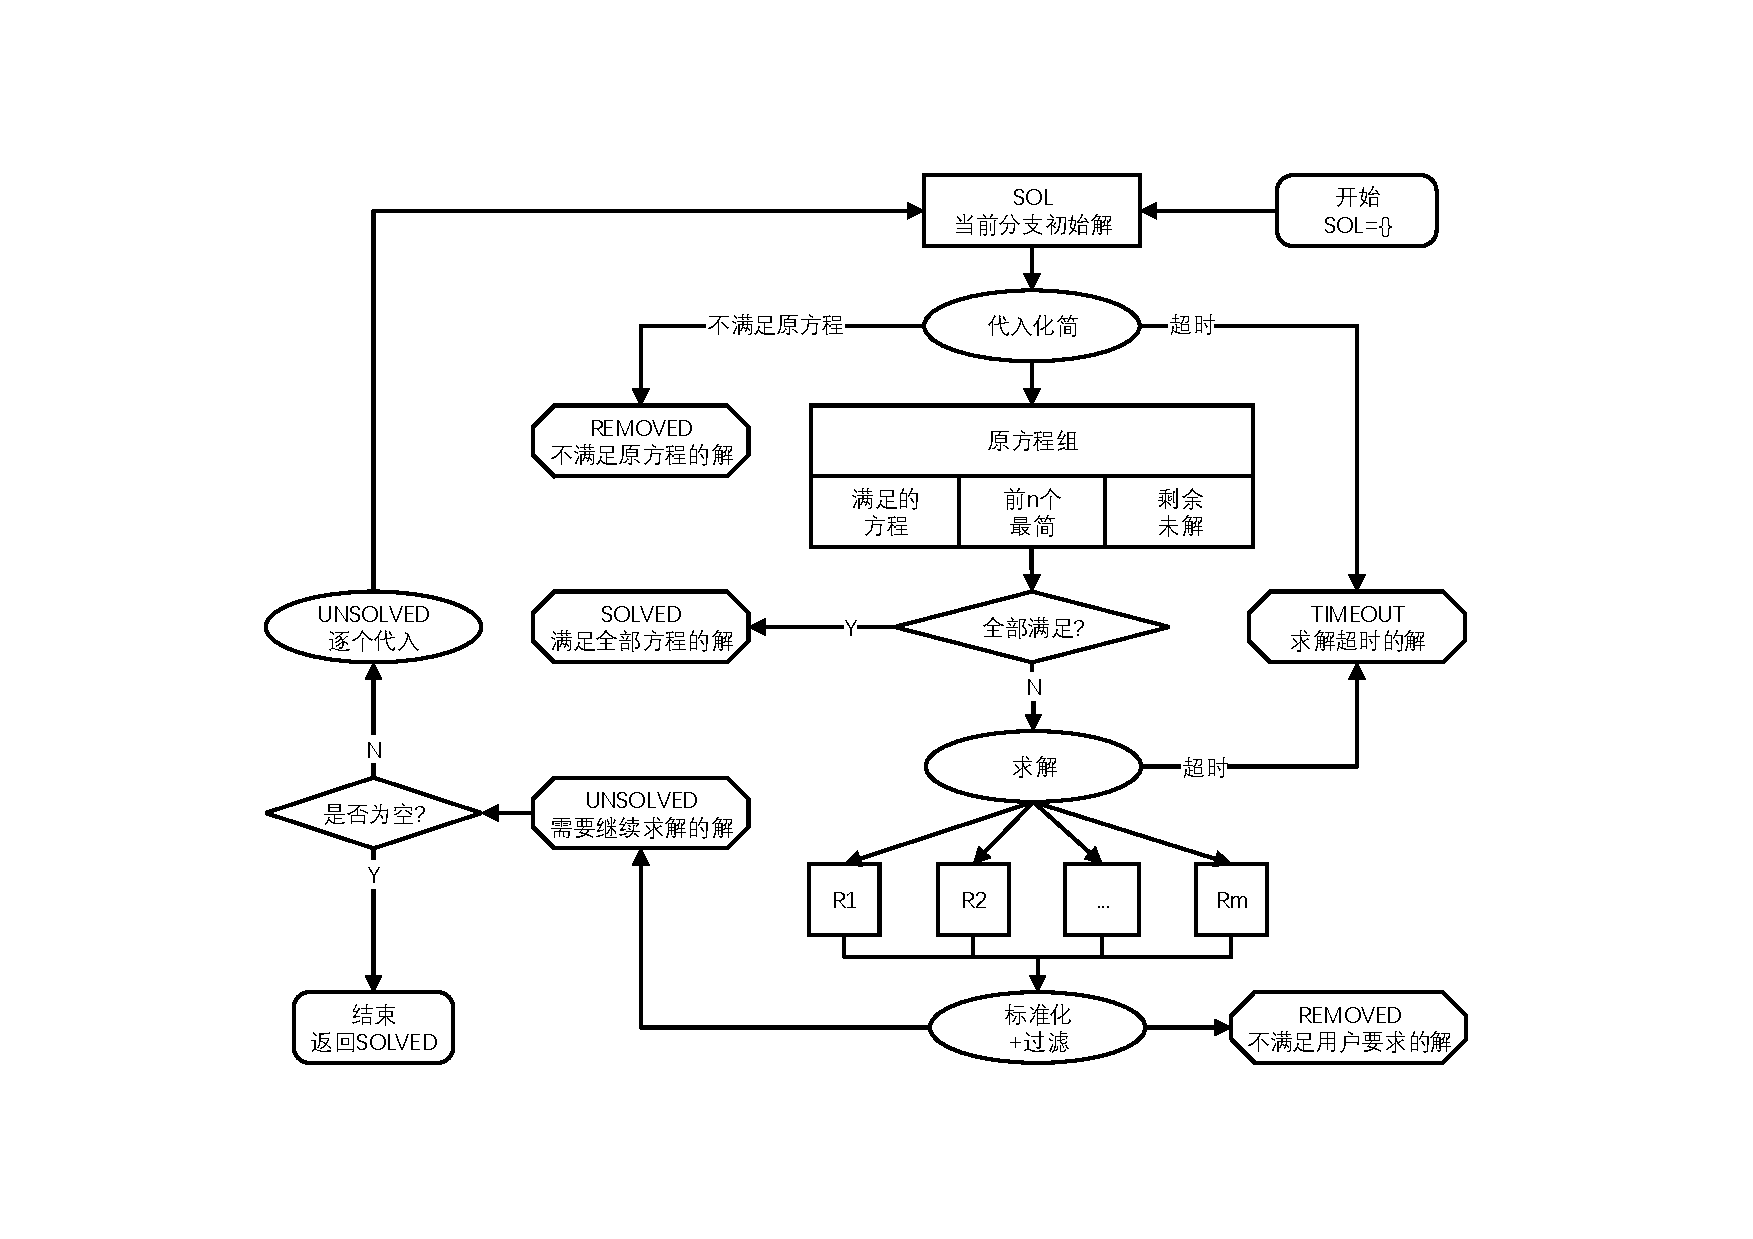
\includegraphics[width=0.9\textwidth]{fig/pgsolve.pdf}
\caption{PGSolve 算法框架}\label{PGSolve}
\end{figure}

该算法的具体步骤如下:
\begin{compactenum}[Step 1.]
\item 初始化: 用于保存解集的 SOLVED\D UNSOLVED 以及 TIMEOUT 三个容器为空集. 令 SOL=\{\}. 
\item 将当前解SOL代入原方程组之后并化简. 化简之后, 原方程组可以分为三个部分. 第一部分是已经满足的方程, 这些方程在代入化简后为零. 将剩余的方程按照复杂度进行升序排序之后, 可以根据用户给定的n分为两个部分. 
\item 在代入化简后, 
    \begin{compactenum}[(a)]
    \item 如果存在一些方程的化简结果为常数, 则表示SOL不满足原方程组, 我们将其废弃后进入下一个分支的求解. 
    \item 若SOL满足原方程组的所有方程, 则将 SOL 加入 SOLVED之后继续下一个分支的求解. 
    \item 若化简超时, 则将 SOL 加入 TIMEOUT 后继续下一个分支的求解. 
    \item 否则, 就取尚未求解的方程中最简单的n个进行求解.
    \end{compactenum}
\item 若求解超时, 则将 SOL 加入 TIMEOUT. 否则, 就对求得的解进行标准化. 标准化包含以下几个步骤:
    \begin{compactenum}[(1)]
    \item 删除每个解中的自由变量. 这是因为 Maple 的 solve 在求解时会返回自由变量(如 x=x).
    \item 将求解结果中的每个解并上 SOL 后构成一个新的方程, 再利用 solve 进行求解, 保证解的最简性和唯一性. 
    \item 再次删除自由变量.
    \item 按照用户指定条件对解进行过滤, 删除不满足用户指定条件的解. 
    \end{compactenum}
\item 标准化之后, 按照用户给定的条件筛选解, 将满足条件的解加入 UNSOLVED 继续求解. 
\item 如果此时 UNSOLVED 为空, 则算法结束, SOLVED 中包含了用户想要的解. 否则, 就将 UNSOLVED 内的元素全部取出之后, 依次作为 SOL 转 Step 2 继续求解. 
\end{compactenum}

在上述算法中, 我们对代入化简后的方程组按照复杂度进行升序排序, 其目的在于降低求解的前$n$个方程所构成的方程组的复杂度.  要想利用分组策略来提高方程组的求解效率, 就需要满足以下两个条件: (1) 前面的分组尽可能的简单, 减少单步的求解时间; (2) 前面的分组解所得的解尽可能的少, 以减小求解分支的数量. 因为这两个条件是互相冲突的, 所以用户需要根据实际求解的情况来指定合适的分组大小. 

一个方程组的复杂度是由三个个方面决定的: 一方面是方程的数量, 方程的数量越多方程组就越复杂; 另一方面是方程组中变量的个数, 变量的个数越多则方程组越复杂; 还有一方面是方程组中表达式的复杂度, 单个表达式长度越长, 次数越高, 则这个表达式越复杂. 出于这些考虑, 按复杂度排序的逻辑如下:
\begin{compactenum}[(1)]
\item 将方程按照变量进行分组, 变量相同的方程放在同一组内.
\item 将上述分组按照变量数量升序排序.
\item 每个分组内利用 Maple 的 \cd{SolveTools:-Complexity} 函数衡量表达式的复杂度, 按照复杂度升序排序.  
\item 上述操作完成后, 将各个分组展开, 把方程组还原为一个列表. 
\end{compactenum}

按照上述策略进行排序就能保证所求解的前$n$个方程构成的方程组是最简的. 接着, 我们就要尽可能地控制解的数量以减少分支的数量. 在变量数目不变的情况下, 一个方程组解的数量和方程的数量相关. 一般而言, 方程数量越多, 约束约苛刻, 则解的数量就越少. 但是方程数量越多, 则求解这个方程组所需要的时间越长. 因此, 求解方程的数量是一个需要权衡的数字, 可以由用户根据实际情况进行设置, 而本文一般取 $n=5$.

此外需要特别说明的是, 我们将SOL代入所有的方程进行代入化简的主要原因如下: 
\begin{compactenum}[(1)]
\item 对尚未求解的方程进行代入化简, 能够对新的方程组按照复杂度重新排序, 从而获得更简单的方程.
\item 对已经求解过的方程进行代入化简, 能够验证当前分支的解是否满足这部分方程. 
\item 虽然我们只求解了部分方程, 但是求得的解可能能够满足全部方程. 将求得的解代入全部方程, 就能根据代入的结果提前结束当前分支的求解, 将当前的解添加到 SOLVED 中. 
\end{compactenum} 

而在 TIMEOUT 中保存超时的解的意义在于, 如果用户在求解结束时愿意花更多的时间来继续求解超时的解, 就可以将 TIMEOUT 赋值给 UNSOLVED, 设定更大的时限重新求解. 

\subsection{并行调度策略} 
在\reffig{PGSolve}所示的算法中, 有三个地方可以并行加速:  
\begin{compactitem}[\textbullet]
\item ``代入化简''所需的时间最长, 而化简一个表达是又是一个工作量比较小的原子任务, 比较适合将其并行化.
\item ``标准化+过滤''所需的时间极短, 并行加速的意义不大.
\item ``UNSOLVED逐个代入''这个步骤的每个子任务所包含的工作量过大, 不适合并行加速.
\end{compactitem}
因此, 我们选择将``代入化简''这一步并行化. 而我们所采用的并行调度策略是经典的Master-Slave调度模型\cite{sahni1996master}. 

如\reffig{msp}所示, Master-Slave 调度模型的原理如下:
\begin{compactenum}[Step 1.]
\item 所有并行任务进入任务池.
\item Master 节点从任务池拉取任务分配给空闲的 Slave 节点, 直到没有空闲节点.
\item Slave 完成任务后返回, Master 将新的任务分配给当前 Slave 节点, 直至所有任务完成. 
\end{compactenum}

\begin{figure}[htbp]
\centering 
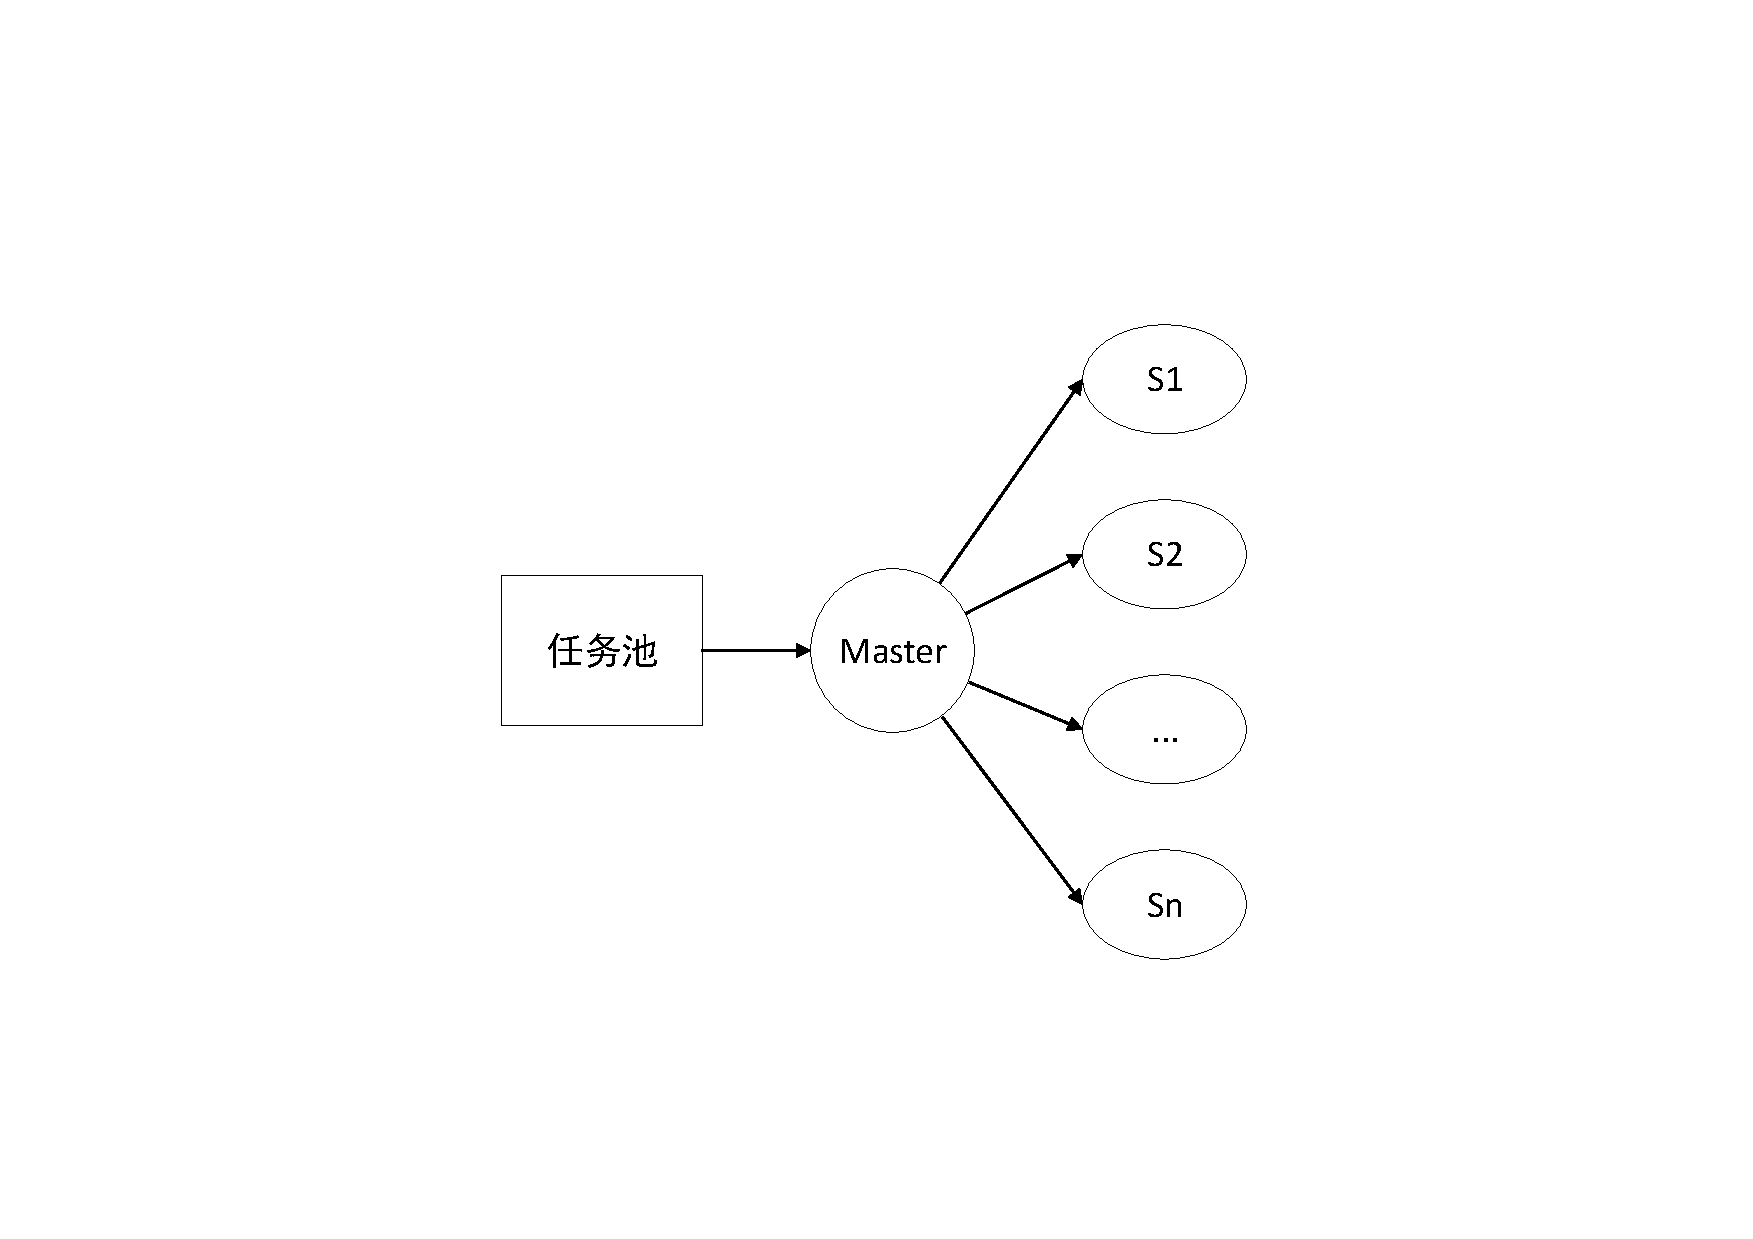
\includegraphics[width=0.5\textwidth]{fig/msp.pdf}
\caption{Master-Slave 调度模型}\label{msp}
\end{figure}

在 Maple 中, 并行可以分为基于 Threads 软件包的多线程并行和基于 Grid 软件包的多进程并行. 多线程并行可以进行资源共享, 但当多个线程同时访问一个资源时会存在线程安全的问题, 有可能导致程序出错. 因为 Maple 中许多重要的内置函数(如, \cd{solve})都不是线程安全的, 因此我们选择采用多进程并行. 多进程并行不存在资源共享的问题, 进程之间的交流靠通信实现. 尽管 Grid 软件包中有 \cd{Map} 这样一个高级接口可以直接实现基于 Master-Slave 调度模型的并行过程, 但是为了控制整个计算过程的时长, 我们还是自行实现了一个 \cd{pmap} 函数. 该函数的调用方式为 \cd{pmap(f,v,TL)}. 其中, \cd{f} 是作用在列表 \cd{v} 中每个元素上的函数, 而 \cd{TL} 则是总的时间限制. PGSolve 中的并行过程就是基于 \cd{pmap} 函数实现的. 

\subsection{PGSolve软件包的接口与实现}
根据上文所述的算法, 我们在 Maple 中实现了 PGSolve 软件包. PGSolve 软件包的核心接口是 \cd{GroupSolver} 对象, 该对象实现了\reffig{PGSolve}所述的功能. \cd{GroupSolver}对象的构造函数为: 
\begin{verbatim}
GroupSolver(eqs,vrs,filter,{use_parallel});
\end{verbatim}
其中, 
\begin{compactitem}[\textbullet]
\item \cd{eqs} 表示方程组;
\item \cd{vrs} 表示需要求解的变量的集合;
\item \cd{filter} 是一个用户自定义的函数, 对需要删除的解返回 \cd{true}, 对需要保留的解返回 \cd{false};
\item 选项 \cd{use\_parallel} 是可选的, 当用户指定这个选项时, \cd{GroupSolver} 才会在求解时采用并行策略进行加速.
\end{compactitem}
当 \cd{GroupSolver} 的构造完成时, 它会将 \cd{eqs, vrs, filter} 作为成员变量进行存储, 同时初始化 SOLVED\D UNSOLVED 和 TIMEOUT 为空集. 

当 \cd{GroupSolver} 构造完成后, 用户就可以调用 \cd{GroupSolver:-agsolve(n,TL)} 实现自动求解, 调用 \cd{GroupSolver:-pgsolve(n,TL)} 实现分步求解. 其中, \cd{n}表示分组求解的个数, 而\cd{TL}表示单步求解的最长时间.  \cd{GroupSolver:-agsolve} 对应实现了\reffig{PGSolve}的全部流程, 而 \cd{GroupSolver:-pgsolve} 实现的则是从``SOL''节点开始到``是否为空?''的流程. 使用 \cd{agsolve} 的优势在于整个求解流程自动完成, 缺点在于不能中途调整 \cd{n} 和 \cd{TL}. 而 \cd{pgsolve} 则可以根据求解情况, 在每一步中设置不同的 \cd{n} 和 \cd{TL} 进行求解. 

\section{求 $n$-孤子和 1-lump 相互作用解的直接代数方法}
在微分方程的求解过程中, 许多方法最终都归结于代数方程组的求解. 包括齐次平衡方法\D 双曲正切方法和 Jacobi椭圆函数方法等, 最终都需要求解代数方程组. 不过这些方法最终的方程组规模都不大, 本文就不以它们举例了. 我们在\refchp{ch02}中, 基于简单 Hirota 方法求得了 NLEE 的孤子解\D 呼吸子解和lump 解. 其实, 我们也能通过直接代数方法来求解它们. 不过, 显然是\refchp{ch02}中的算法求解方法效率更高. 但是, 对于孤子解和lump解的相互作用解, 目前只能利用直接代数方法进行求解. 由于求解该方法能够产生大规模的代数方程组, 我们就以它为例来展示 PGSolve 的作用, 同时测试 PGSolve 的有效性. 

采用直接代数方法求 $n$-孤子和 1-lump 相互作用解的第一步和\refchp{ch02}中的简单 Hirota 方法一样, 都是利用 \Painleve{}展开方法确定变换. 然后, 若自变量为$x_1,\cdots,x_m$, 则解的假设形式为
\begin{equation}
f_n=\sbrace{\xi_1+\eta_1}^2+\sbrace{\xi_2+\eta_2}^2+\sum_{i=1}^{2^n}\sbrace {q_i\prod_{k \in P_i}{\exp(\xi_{k+2})}}. \label{f-ns1l}
\end{equation}
其中, $P_i$ 是 $\bbrace{1,\cdots,n}$的全体子集中的第$i$个, 而
\begin{equation}
\xi_k=\sum_{j=1}^m{p_{j,k}x_j}.
\end{equation}
在\refeqn{f-ns1l}中, 前两个平方项的和构成了lump解的部分, 而最后一个求和项则是孤子解的部分. 在该假设形式中, 待定参数的集合为
\begin{equation}
    \bbrace{q_i|1\le i \le 2^n} \cup \bbrace{p_{j,k}|1\le j \le m, 1\le k \le n+2} \cup \bbrace{\eta_1,\eta_2}. 
\end{equation}

值得说明的是, 本文是在\refchp{ch02}中多孤子解的生成公式(\ref{f-soliton-new})的基础上给出\refeqn{f-ns1l}的. \refeqn{f-ns1l}的优点在于: 当高阶的解在某些参数取零时, 能够退化为相同形式的低阶解. 例如,
\begin{equation}
    f_1=\sbrace{\xi_1+\eta_1}^2+\sbrace{\xi_2+\eta_2}^2+q_1+q_2 \exp(\xi_3)
\end{equation}
在取$q_2=0$时, 可以退化为
\begin{equation}
    f_0=\sbrace{\xi_1+\eta_1}^2+\sbrace{\xi_2+\eta_2}^2+q_1.
\end{equation}
要想达到上述效果, 就需要对 $\bbrace{1,\cdots,n}$ 的全体子集进行合适的排序. 事实上, 按照\refalg{allsubset}生成的子集能够满足上述要求. 在\refalg{allsubset}中, 我们假设并集操作会保留元素的顺序. 

\begin{algorithm}
\caption{NS1L中的全体子集生成算法}\label{allsubset}
\Fn{$allsubset(n)$}{
    \lIf{$n=0$}{
        \Return{$\bbrace{\emptyset}$}
    }
    $X\gets allsubset(n-1)$\;
    \Return{$X \cup  \sbrace{\bigcup\limits_{v\in X}{v \cup \{n\}}}$}\;
}
\end{algorithm}

在确定了解的假设形式之后, 我们需要确定参数的约束条件. 按照相互作用解的实际意义, 需要满足:
\begin{compactenum}[(1)]
\item 孤子解的各个组成部分非零. 即$q_i\neq 0~(i=1,\cdots,2^n)$.
\item lump 的各个组成部分非零, 即$\xi_1\neq 0,\xi_2\neq 0$.
\item 孤子解的各个孤子非零, 即$\xi_k\neq 0~(k=3,\cdots,n+2)$.
\item 孤子解和lump解的维数不能退化, 即自变量的数量不能减少. 
\end{compactenum}

为了筛选出满足上述条件的解, 我们提出一个\emph{避免取值集合}的概念. 给定一个\emph{避免取值集合}$S$, 对于原方程组的一个解$t$ (是一个集合), 若存在$s\in S$, 满足$s\subseteq t$, 则$t$就不是我们想要的解. 而在我们的问题中, 
\begin{equation}
\begin{split}
    S&=\bbrace{\bbrace{q_i=0}|1\le i \le 2^n} \\ 
     &\cup \bbrace{\bbrace{p_{1,k}=0,\cdots,p_{m,k}=0}|1\le k \le n+2}  \\
     &\cup \bbrace{\bbrace{p_{j,1}=0,p_{j,2}=0}|1\le j \le m} \\ 
     &\cup \bbrace{\bbrace{p_{j,3}=0,\cdots,p_{j,n+2}=0}|1\le j \le m} . 
\end{split}
\end{equation}
式中第一个集合保证了孤子解的各个组成部分非零, 第二个集合保证了各个孤子非零以及lump解的各个部分非零, 第三个集合保证了lump解部分的维数不退化, 而第四个集合保证了孤子解部分的维数不退化.

\section{NS1L 和 PGSolve 软件包的应用实例}
基于上一节中的理论分析, 结合本文在 PAnalyze 和 PGSolve 软件包上的工作, 我们开发了能够求解非线性演化方程 $n$-孤子和 1-lump 相互作用解的软件包 NS1L. 下面, 本文将展示 NS1L 的调用方式, 同时测试 PGSolve 的求解性能. 此外, 在下文中, 我们将简称 n-孤子和 1-lump 的相互作用解为 nS-1L 解. 

\subsection{基本用法}
考虑(3+1)YTSF方程\CITEcaYTSF,
\begin{equation}
    3\,\alpha\,u_{{{\it yy}}}+4\,u_{{x}}u_{{{\it xz}}}+2\,u_{{{\it xx}}}u_{{z}}-4\,u_{{{\it tx}}}+u_{{{\it xxxz}}}=0. 
\end{equation}

因为NS1L中也可以取$n=0$, 所以我们先以0S-1L解(即 lump 解)为例进行求解. 

Step 1. 生成代数方程组.
\begin{verbatim}
sh:=gen_eq(eq,0,p,q);
\end{verbatim}
这里, \cd{gen\_eq} 的第一个参数是一个NLEE, 第二个参数\cd{n}表示相互作用解中孤子解的阶数. 而\cd{p,q}则对应\refeqn{f-ns1l}中的$p,q$, 用于给待定参数设置变量名. 此外, 和 TwSolver 一样, NS1L 的求解也涉及了\Painleve{}展开方法的相关计算, 所以也存在多解的情况. 所以, \cd{gen\_eq}也可以指定\cd{select\_solution}参数来人工选择 TPE 的解. 最后, 返回值\cd{sh}是一个\cd{EqnHolder}对象. 该对象的作用类似于TwSolver中的\cd{SolHolder}对象, 我们接下来将一一展示它的作用. 

Step 2. 求解代数方程组.
\begin{verbatim}
ph:=sh:-get_solver();
sols:=ph:-agsolve(5);
\end{verbatim}
这里的第一行我们先利用\cd{EqnHolder}对象获得求解对应代数方程组的\cd{GroupSolver}对象. 其实, 我们还能通过\cd{sh:-get\_solver(use\_parallel)}来获得使用并行策略进行加速的\cd{GroupSolver}对象. 第二行调用PGSolve中的\cd{GroupSolver}对象进行代数方程组的求解. 在求 0S-1L 解时, 共有35个方程和11个待定参数, \cd{GroupSolver}能够在1秒左右求得3组解. 对于这个例子, PGSolve 在求解时的分支图如\reffig{sb0}所示. 

\begin{figure}[htbp]
\centering
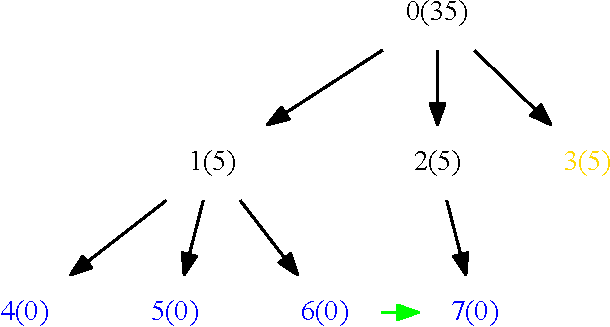
\includegraphics[width=.3\textwidth]{fig/0S1L.pdf}
\caption{(3+1)YTSF-0S1L 求解分支图}\label{sb0}
\end{figure}

本文的求解分支图是在求解过程中将解的类型和关系按照 GraphViz\cite{ellson2001graphviz} 的相关格式输出到文件之后, 调用 GraphViz 生成的. 在求解分支图中, 每个节点的格式为``解的编号(代入该解后剩余的方程数)''. 节点的颜色表示解的类型, 解的类型有四种, 和\reffig{PGSolve}保持一致. 黑色表示 UNSOLVED 的解, 蓝色表示 SOLVED 的解, 黄色表示 REMOVED 的解, 红色表示 TIMEOUT 的解. 绿色的箭头表示等价的解, 蓝色箭头表示一个解是另一个解的特解. 这里的等价指的是表达式形式相同. 而特解的定义为: 如果解A是解B的子集, 则解B是解A的特解. 

在\reffig{sb0}中, 0号解是空集, 此时剩余35个方程. 第一轮求解之后, 生成了编号为1,2的两个解. 此时, 未解的方程只有5个. 也就是说, 虽然我们在求解时只求解了5个方程, 但是解得的解满足了30个方程. 这就 PGSolve 效率高于传统求解算法的主要原因. 在第二轮求解时, 我们发现2号解不是原方程的解, 而1号解则生成了3个原方程的解. 

Step 3. 消除等价的解.
\begin{verbatim}
sols:=sh:-sh:-filter_sol(sols);
\end{verbatim}
在\cd{GroupSolver}求解完成时, 已经消除了一般意义下的等价解和特解. 但是在本节的问题中, 交换lump解部分的$\xi_1+\eta_1$和$\xi_2+\eta_2$, 虽然得到的两个解在代数意义下是不同的, 但实际上它们是等价的. 于是, 我们在\cd{EqnHolder}对象中加入了\cd{filter\_sol}函数来解决该问题. 在这个例子中, 原本的3个解被精简为2个解, 它们分别是
\begin{equation}
\left\{ 
\begin{split}
&p_{{31}}={\frac {p_{{11}}p_{{32}}}{p_{{12}}}}, 
p_{{41}}={\frac {3\alpha \left(  \left( {p_{{21}}}^{2}-{p_{{22}}}^{2} \right) p_{{11}}+2p_{{12}}p_{{21}}p_{{22}} \right) }{4{p_{{11}}}^{2}+4{p_{{12}}}^{2}}}, \\
&p_{{42}}={\frac {3\alpha \left( 2p_{{11}}p_{{21}}p_{{22}}-p_{{12}}{p_{{21}}}^{2}+p_{{12}}{p_{{22}}}^{2}\right) }{4{p_{{11}}}^{2}+4{p_{{12}}}^{2}}}, 
q_{{1}}=-{\frac {p_{{32}} \left( {p_{{11}}}^{2}+{p_{{12}}}^{2} \right) ^{3}}{\alpha p_{{12}} \left( p_{{11}}p_{{22}}-p_{{12}}p_{{21}} \right) ^{2}}} 
\end{split}
\right\}  
\label{0S1L-1}
\end{equation}
和
\begin{equation}
 \left\{ p_{{12}}=0,p_{{31}}=-{\frac {\alpha q_{{1}}{p_{{22}}}^{2}
}{{p_{{11}}}^{3}}},p_{{32}}=0,p_{{41}}={\frac {3\alpha
 \left( {p_{{21}}}^{2}-{p_{{22}}}^{2} \right) }{4p_{{11}}}},p_{{42}
}={\frac {3\alpha p_{{21}}p_{{22}}}{2p_{{11}}}} \right\} . \label{0S1L-2}
\end{equation}

Step 4. 获取解的表达式.

类似于TwSolver, NS1L中的\cd{EqnHolder}对象也提供了获取解的功能. \cd{get\_sol}能够获得原方程的解, \cd{get\_fsol}能够获得经过TPE变换后的方程的解. 例如
\begin{verbatim}
sh:-get_fsol(sols[2]);
\end{verbatim}
能够获得\refeqn{0S1L-2}对应的解 
\begin{equation}
\sbrace{p_{11}x+p_{21}y+\frac{p_{22}^2q_1\alpha}{p_{11}^3}z+\frac{3\alpha (p_{21}^2-p_{22}^2)}{4p_{11}}t+p_{51}}^2
+\sbrace{p_{22}y+\frac{3\alpha p_{21}p_{22}}{2p_{11}}t+p_{52}}^2+q_1 .
\end{equation}
需要说明的是, 在NS1L中, $p_{m+1,1},p_{m+1,2}$分别对应\refeqn{f-ns1l}中的$\eta_1,\eta_2$, 其中$m$是方程的维数. 

Step 5. 验证解.
\begin{verbatim}
sh:-verify_sol(sols[1]);
\end{verbatim}
NS1L也提供了验证解的功能, \cd{verify\_sol}的输入参数为形如\refeqn{0S1L-1}的参数关系的解集. 验证方法是将\cd{get\_sol}的结果代入到原方程中进行验证. 要对\cd{sols}中所有的解都进行验证, 也可以调用\cd{map(sh:-verify\_sol,[sols[]])}. 经验证, \refeqn{0S1L-1}和\refeqn{0S1L-2}都是原方程的解. 因为 NS1L 所输出的解一定满足代数方程组, 所以也可以省略这一步.

Step 6. 绘制解. 例如
\begin{verbatim}
sh:-plot_sol(
    sols0[1],
    [x=-30..30,y=-30..30,alpha=1,t=0,z=0,p[2,1]=-1,p[3,2]=-1],
    rest_assign,
    grid=[100,100],orientation=[-78,60,-3],view=-1.6..1.6
);
\end{verbatim}
能够得到如\reffig{fig-0s1l-1}所示的结果. 在\cd{plot\_sol}中, 第一个参数是解, 第二个参数是绘制时的参数取值范围, 选项\cd{rest\_assign}表示将未赋值的参数默认取为1, 剩下的参数是 \cd{plot3d} 的参数, 用于调整绘制结果的外形. 对于\refeqn{0S1L-2}所对应的解, 设参数的取值范围为 \cd{[x=-30..30,y=-30..30,alpha=1,t=0,z=0]}, 指定\cd{rest\_assign}选项, 则可以得到如\reffig{fig-0s1l-2}所示的结果.

\begin{figure}[htbp]
\centering
\subfigure[\refeqn{0S1L-1}对应的解 \label{fig-0s1l-1}]{
    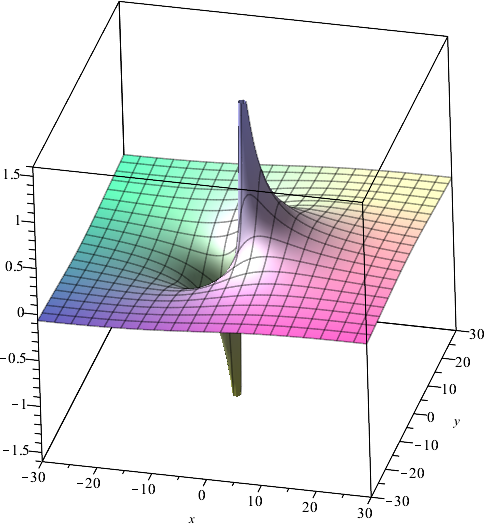
\includegraphics[width=.3\textwidth]{fig/0S1L-1.png}
}
\subfigure[\refeqn{0S1L-2}对应的解 \label{fig-0s1l-2}]{
    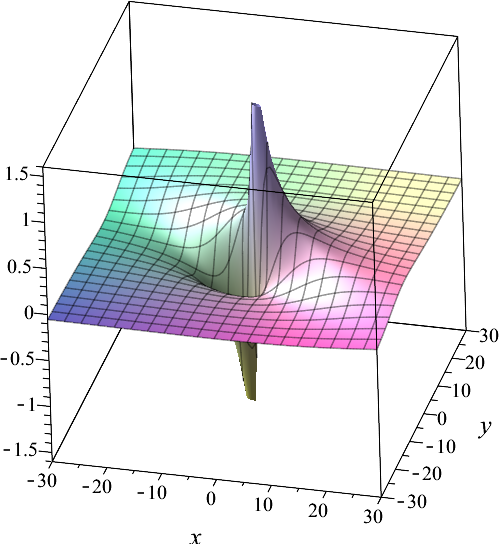
\includegraphics[width=.3\textwidth]{fig/0S1L-2.png}
}
\subfigure[\refeqn{0S1L-3}对应的解 \label{fig-0s1l-3}]{
    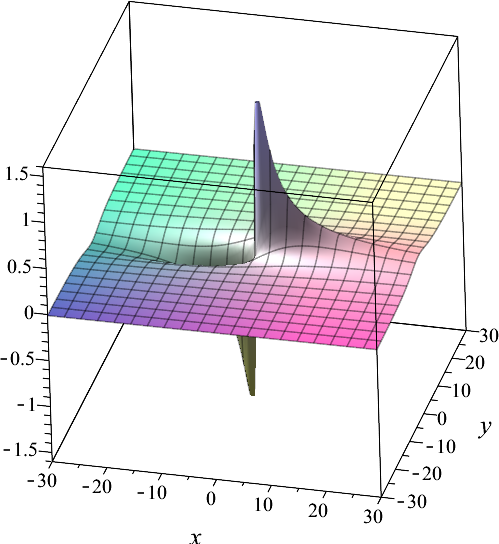
\includegraphics[width=.3\textwidth]{fig/0S1L-3.png}
}
\caption{(3+1)JM 方程的 0S-1L 解}
\end{figure}

综上, 我们已经展示了使用 NS1L 进行求解的一般流程. 

此外, 因为我们以lump解为例进行了求解, 而 TwSolver 也能求 lump 解, 于是我们就来探索一下两种方式得到的解有什么不同. 

由\reftab{verify}可知, (3+1)YTSF方程在$\PS=\bbrace{1,3}$时能通过 TwSolver 得到 lump 解. 调用
\begin{verbatim}
TwSolver:-twsolve(eq,{1,3},PL=[a,b,c,d])
\end{verbatim}
并对计算结果进行代换
\begin{equation}
    b_{1,RE}=\beta,b_{1,IM}=\gamma,c=\delta,
\end{equation}
可以得到lump解
\begin{equation}
    f=\sbrace{x+\beta y + \delta z+ \frac{3\alpha (\beta^2-\gamma^2)}{4}t}^2+\sbrace{\gamma y+\frac{3\alpha \beta \gamma}{2}t}^2-\frac{\delta}{\alpha \gamma^2}. \label{0S1L-3}
\end{equation}
取\cd{[x=-30..30,y=-30..30,alpha=1,t=0,z=0,beta=1/2,gamma=4]}进行绘图, 可以得到\reffig{fig-0s1l-3}. 

经过计算, 我们发现, 当
\begin{equation}
\left\{ 
\begin{array}{l}
p_{11}=\sqrt{1-p_{12}^2},
p_{22}=\beta p_{12}+\gamma p_{11},
p_{21}=\frac{p_{12}(p_{22}-\beta)}{p_{11}},  
p_{32}=\delta p_{12},p_{51}=p_{52}=0
\end{array}
\right\}
\end{equation}
时, \refeqn{0S1L-1}所对应的解能够转化为\refeqn{0S1L-3}. 也就是说, 直接代数方法得到的 lump 解比简单 Hirota 方法得到的解更加具有一般性. 

\subsection{直接求解与继承求解}

接下来, 我们将求解(3+1)YTSF方程的 1S-1L 解. 按照之前的步骤, 我们调用如下代码进行求解. 
\begin{verbatim}
sh:=gen_eq(eq,1,p,q);
ph:=sh:-get_solver(use_parallel);
sols:=sh:-filter_sol(ph:-agsolve(5));
\end{verbatim}

在求解时, 我们得到了一个具有16个变量和120个方程的代数方程组. 在求解时, 我们开启了并行加速. 对于这120个方程, 在10秒左右就得到了3个不同的相互作用解. 我们称这种求解方法为\emph{直接求解}.

事实上, 因为在我们假设形式中 1S-1L 解包含了 0S-1L 解, 所以我们也可以将 0S-1L 解作为初始解进行求解. 这种方法被称为\emph{继承求解}. 继承求解的调用方式为
\begin{verbatim}
sh:=gen_eq(eq,1,p,q);
ph:=sh:-get_solver(use_parallel);
ph:-set_init_sols(sols0);
sols:=sh:-filter_sol(ph:-agsolve(5));
\end{verbatim}
其中, \cd{sols0}表示之前求得的两个 0S-1L 解. 继承求解的关键命令就是在求解开始前, 调用\cd{set\_init\_sols}函数来设置初始解. 按照上述方法进行求解, 在5秒左右获得了3个不同的相互作用解. 经过验证, 这3个解和继承求得的3个解是等价的.

我们可以在\reffig{sb1}中对比直接求解和继承求解的分支图. 在直接求解时, 经历了5轮求解得到3个解, 期间一共计算了14个解. 在继承求解时, 经历4轮求解得到了3个解, 期间一共计算了11个解. 显然, 继承求解的分支比直接求解更少. 不管是直接求解还是继承求解, 它们都迅速地将方程数量从120降至16, 这就是 PGSolve 能够迅速求解大规模方程的主要原因. 此外, 在\reffig{sb1-d}中还能看到一个绿色的箭头, 这表示10号解等价于7号解, 在求解过程中将 10 号解从 UNSOLVED 中删除, 可以避免重复求解, 减少运行时间. 

\begin{figure}[htbp]
\centering
\subfigure[直接求解的分支图 \label{sb1-d}]{
    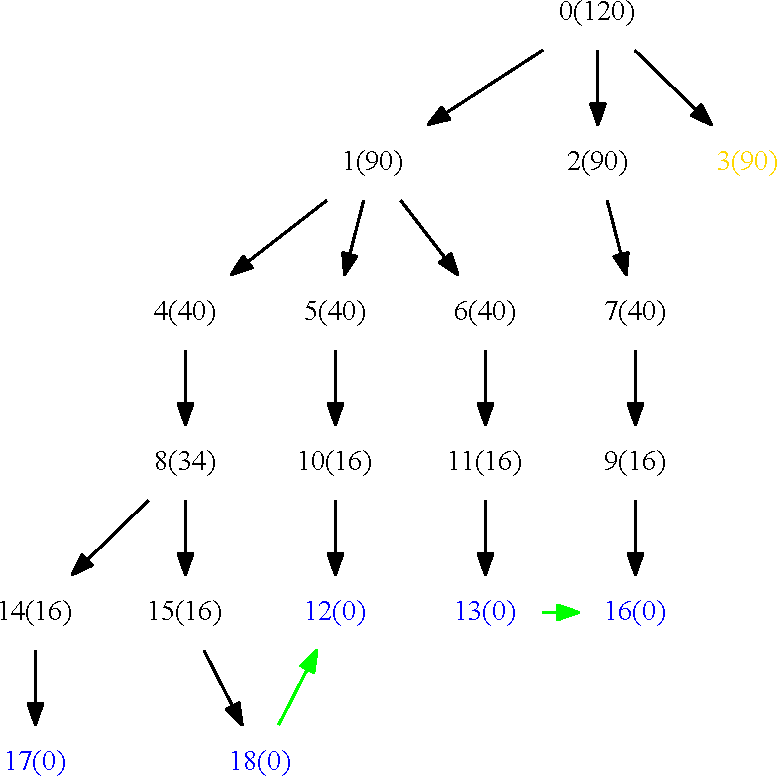
\includegraphics[width=.5\textwidth]{fig/1S1L-dir.pdf}
}
\hfill
\subfigure[继承求解的分支图 \label{sb1-e}]{
    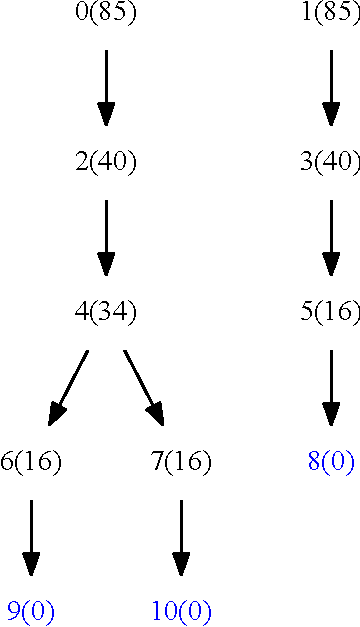
\includegraphics[width=.35\textwidth]{fig/1S1L-ext.pdf}
}
\caption{1S-1L的直接求解与继承求解对比图} \label{sb1}
\end{figure}

为了简化解的表示, 同时也为了能够和\citett{zhangYTSF}中的结果进行对比, 我们取解的假设形式为
\begin{equation}
\begin{split}
    f&=(a_1 x+a_2 y+a_3 z+ a_4 t +a_5)^2+(a_6 x+a_7 y+a_8 z+ a_9 t +a_{10})^2 \\
    &+b+k \exp(k_1 x + k_2 y +k_3 z+ k_4 t).
\end{split}
\end{equation}

NS1L得到的三个解为
\begin{eqnarray}
\renewcommand{\arraystretch}{1.2}
\left\{
\begin{array}{l}
b=\frac{\left( {{{a}_{1}}}^{2}+{{{a}_{6}}}^{2}\right) }{{{{k}_{1}}}^{2}},
{{a}_{2}}=\frac{\left( {{{a}_{1}}}^{2}\,{{k}_{2}}+{{{a}_{6}}}^{2}\,{{k}_{2}}-{{a}_{6}}\,{{k}_{1}}\,{{a}_{7}}\right) }{{{a}_{1}}\,{{k}_{1}}},
{{a}_{3}}=-\frac{\alpha\,\left( {{a}_{6}}\,{{k}_{2}}-{{a}_{7}}\,{{k}_{1}}\right) ^{2}}{{{a}_{1}}\,{{{k}_{1}}}^{4}},\\
{{a}_{4}}=\frac{3\,\alpha\,\left( {{{a}_{1}}}^{2}\,{{{k}_{2}}}^{2}+{{{a}_{6}}}^{2}\,{{{k}_{2}}}^{2}-{{{k}_{1}}}^{2}\,{{{a}_{7}}}^{2}\right) }{4\,{{{k}_{1}}}^{2}\,{{a}_{1}}},
{{a}_{8}}=-\frac{{{a}_{6}}\,\alpha\,\left( {{a}_{6}}\,{{k}_{2}}-{{a}_{7}}\,{{k}_{1}}\right) ^{2}}{{{{a}_{1}}}^{2}\,{{{k}_{1}}}^{4}},\\
{{k}_{3}}=-\frac{\alpha\,\left( {{a}_{6}}\,{{k}_{2}}-{{a}_{7}}\,{{k}_{1}}\right) ^{2}}{{{{a}_{1}}}^{2}\,{{{k}_{1}}}^{3}},
{{k}_{4}}=\frac{\alpha\,\left( 3\,{{{a}_{1}}}^{2}\,{{{k}_{2}}}^{2}-{{{a}_{6}}}^{2}\,{{{k}_{2}}}^{2}+2\,{{a}_{6}}\,{{a}_{7}}\,{{k}_{1}}\,{{k}_{2}}-{{{k}_{1}}}^{2}\,{{{a}_{7}}}^{2}\right) }{4\,{{{a}_{1}}}^{2}\,{{k}_{1}}},\\
{{a}_{9}}=-\frac{3\,\alpha\,\left( {{{a}_{1}}}^{2}\,{{a}_{6}}\,{{{k}_{2}}}^{2}-2\,{{{a}_{1}}}^{2}\,{{a}_{7}}\,{{k}_{1}}\,{{k}_{2}}+{{{a}_{6}}}^{3}\,{{{k}_{2}}}^{2}-2\,{{{a}_{6}}}^{2}\,{{a}_{7}}\,{{k}_{1}}\,{{k}_{2}}+{{a}_{6}}\,{{{a}_{7}}}^{2}\,{{{k}_{1}}}^{2}\right) }{4\,{{{a}_{1}}}^{2}\,{{{k}_{1}}}^{2}}\\
\end{array}
\right\}, \label{1S1L-1}
\end{eqnarray}
\begin{equation}
\renewcommand{\arraystretch}{1.2}
\left\{
\begin{array}{l}  
b=\frac{{{{a}_{2}}}^{2}}{{{{k}_{2}}}^{2}},
{{a}_{3}}=-\frac{\alpha\,{{{a}_{2}}}^{2}\,{{{a}_{7}}}^{2}}{{{{a}_{1}}}^{3}\,{{{k}_{2}}}^{2}},
{{a}_{4}}=\frac{3\,\alpha\,\left( {{{a}_{2}}}^{2}-{{{a}_{7}}}^{2}\right) }{4\,{{a}_{1}}},
{{a}_{6}}=0,
{{a}_{8}}=0,\\
{{a}_{9}}=\frac{3\,\alpha\,{{a}_{2}}\,{{a}_{7}}}{2\,{{a}_{1}}},
{{k}_{1}}=\frac{{{a}_{1}}\,{{k}_{2}}}{{{a}_{2}}},
{{k}_{3}}=-\frac{{{a}_{2}}\,\alpha\,{{{a}_{7}}}^{2}}{{{{a}_{1}}}^{3}\,{{k}_{2}}},
{{k}_{4}}=\frac{\alpha\,{{k}_{2}}\,\left( 3\,{{{a}_{2}}}^{2}-{{{a}_{7}}}^{2}\right) }{4\,{{a}_{1}}\,{{a}_{2}}}
\end{array}
\right\} \label{1S1L-2}
\end{equation}
和
\begin{equation}
\renewcommand{\arraystretch}{1.2}
\left\{
\begin{array}{l}  
b=\frac{{{{a}_{6}}}^{2}}{{{{k}_{1}}}^{2}},
{{a}_{1}}=0,
{{a}_{3}}=0,
{{a}_{4}}=\frac{3\,\alpha\,{{a}_{2}}\,{{k}_{2}}}{2\,{{k}_{1}}},
{{a}_{7}}=\frac{{{a}_{6}}\,{{k}_{2}}}{{{k}_{1}}},
{{a}_{8}}=-\frac{\alpha\,{{{a}_{2}}}^{2}}{{{{k}_{1}}}^{2}\,{{a}_{6}}},\\
{{a}_{9}}=-\frac{3\,\alpha\,\left( {{{a}_{2}}}^{2}\,{{{k}_{1}}}^{2}-{{{a}_{6}}}^{2}\,{{{k}_{2}}}^{2}\right) }{4\,{{{k}_{1}}}^{2}\,{{a}_{6}}},
{{k}_{3}}=-\frac{\alpha\,{{{a}_{2}}}^{2}}{{{k}_{1}}\,{{{a}_{6}}}^{2}},
{{k}_{4}}=-\frac{\alpha\,\left( {{{a}_{2}}}^{2}\,{{{k}_{1}}}^{2}-3\,{{{a}_{6}}}^{2}\,{{{k}_{2}}}^{2}\right) }{4\,{{k}_{1}}\,{{{a}_{6}}}^{2}}
\end{array}
\right\}. \label{1S1L-3}
\end{equation}

经验证发现, \refeqn{0S1L-1}对应的解和\citett{zhangYTSF}中的解是等价的. 也就是说, NS1L得到的解更加全面. 

对于上述三个解, 取$a_2=2,k=1/3,t=0,z=0$, 其它参数取1, 可以得到如\reffig{fig-1S1L}所示的三个解. 

\begin{figure}[htbp]
\centering
\subfigure[\refeqn{1S1L-1}对应的解]{
    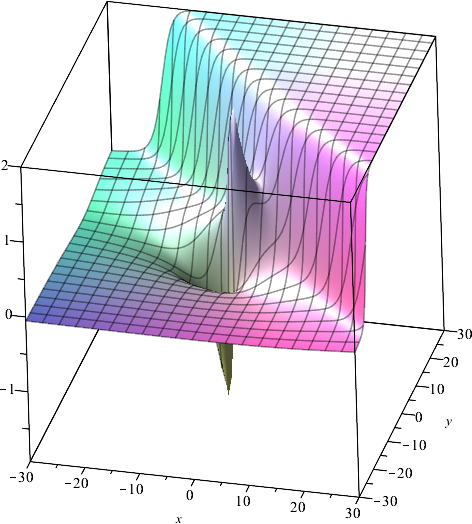
\includegraphics[width=.3\textwidth]{fig/1S1L-1.png}
}
\subfigure[\refeqn{1S1L-2}对应的解]{
    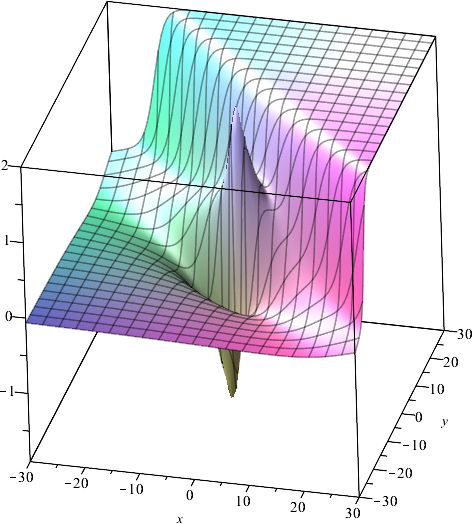
\includegraphics[width=.3\textwidth]{fig/1S1L-2.png}
}
\subfigure[\refeqn{1S1L-3}对应的解]{
    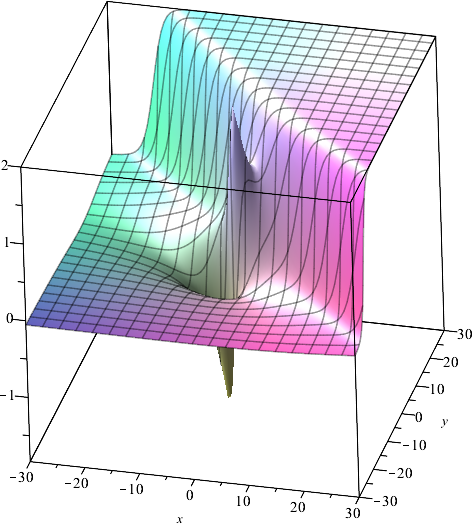
\includegraphics[width=.3\textwidth]{fig/1S1L-3.png}
}
\caption{(3+1)JM 方程的 1S-1L 解} \label{fig-1S1L}
\end{figure}

从\reffig{fig-1S1L}可以看出, 在相同的参数条件下, 3个解存在细微的差别, 但它们都是一个扭状孤子和lump解相互作用的结果. 

最后, 我们来求 2S-1L 解. 通过
\begin{verbatim}
sh:=gen_eq(eq,2,p,q);
ph:=sh:-get_solver(use_parallel);
\end{verbatim}
可以得到一个具有22个变量和324个方程的方程组. 

采用继承求解的方式, 我们在8核CPU (Intel Core i7-7700K @ 4.2GHz) 的硬件条件下, 用时 36 秒, 解得3个解. 该过程的求解分支图如\reffig{sb2-e}所示. 从图中可以看出, 以 1S-1L 的三个解为初始解, 方程的个数迅速地从202个降为7个, 在第5轮求解中得到了3个解. 

\begin{figure}[htbp]
\centering
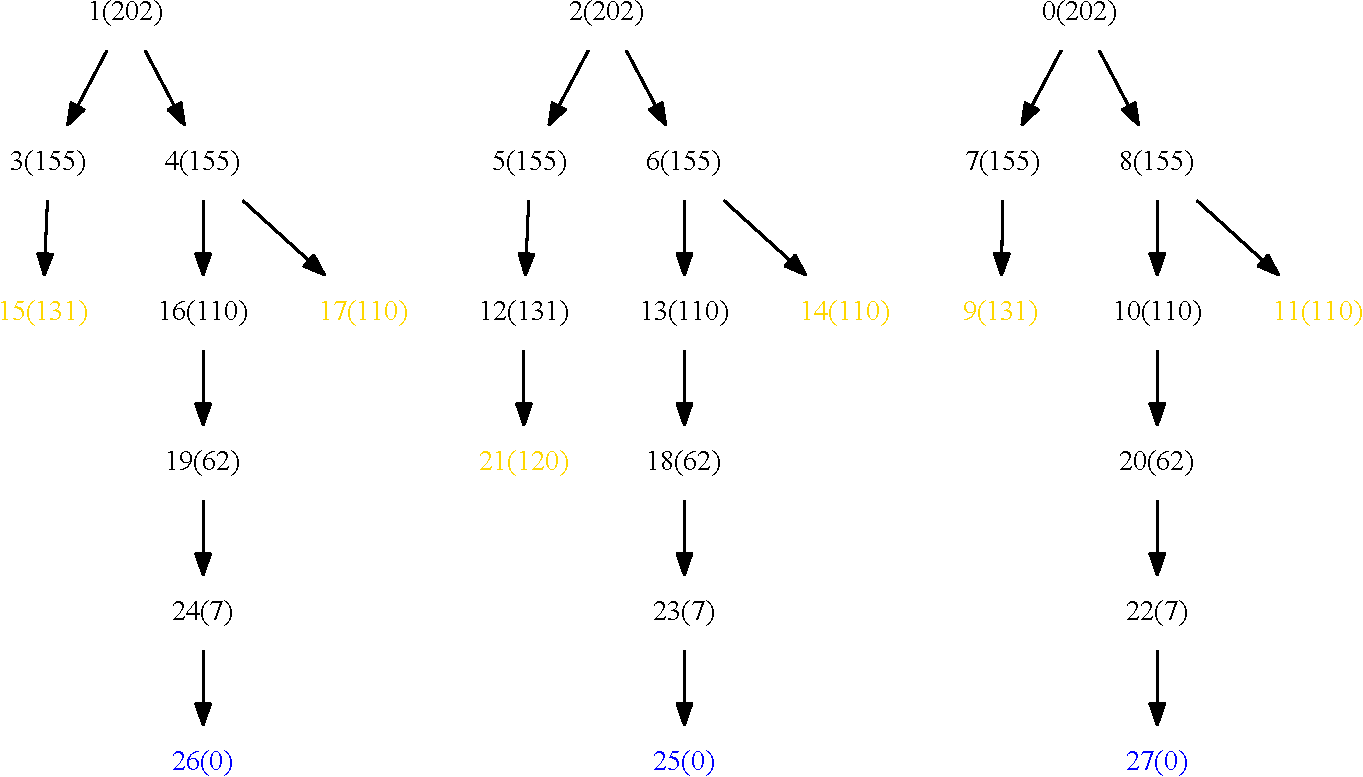
\includegraphics[width=\textwidth]{fig/2S1L-ext.pdf}
\caption{2S-1L 继承求解的分支图}\label{sb2-e}
\end{figure}

而采用直接求解的方式, 设置单步最大时长为100,秒, 最终运行时间430秒, 得到了5个解, 其求解分支图如\reffig{sb2-d}所示. 可以看出求解的分支明显增多, 求解时的增根也明显增多, 还出现了一个求解超时的解.  

\begin{figure}[htbp]
\centering
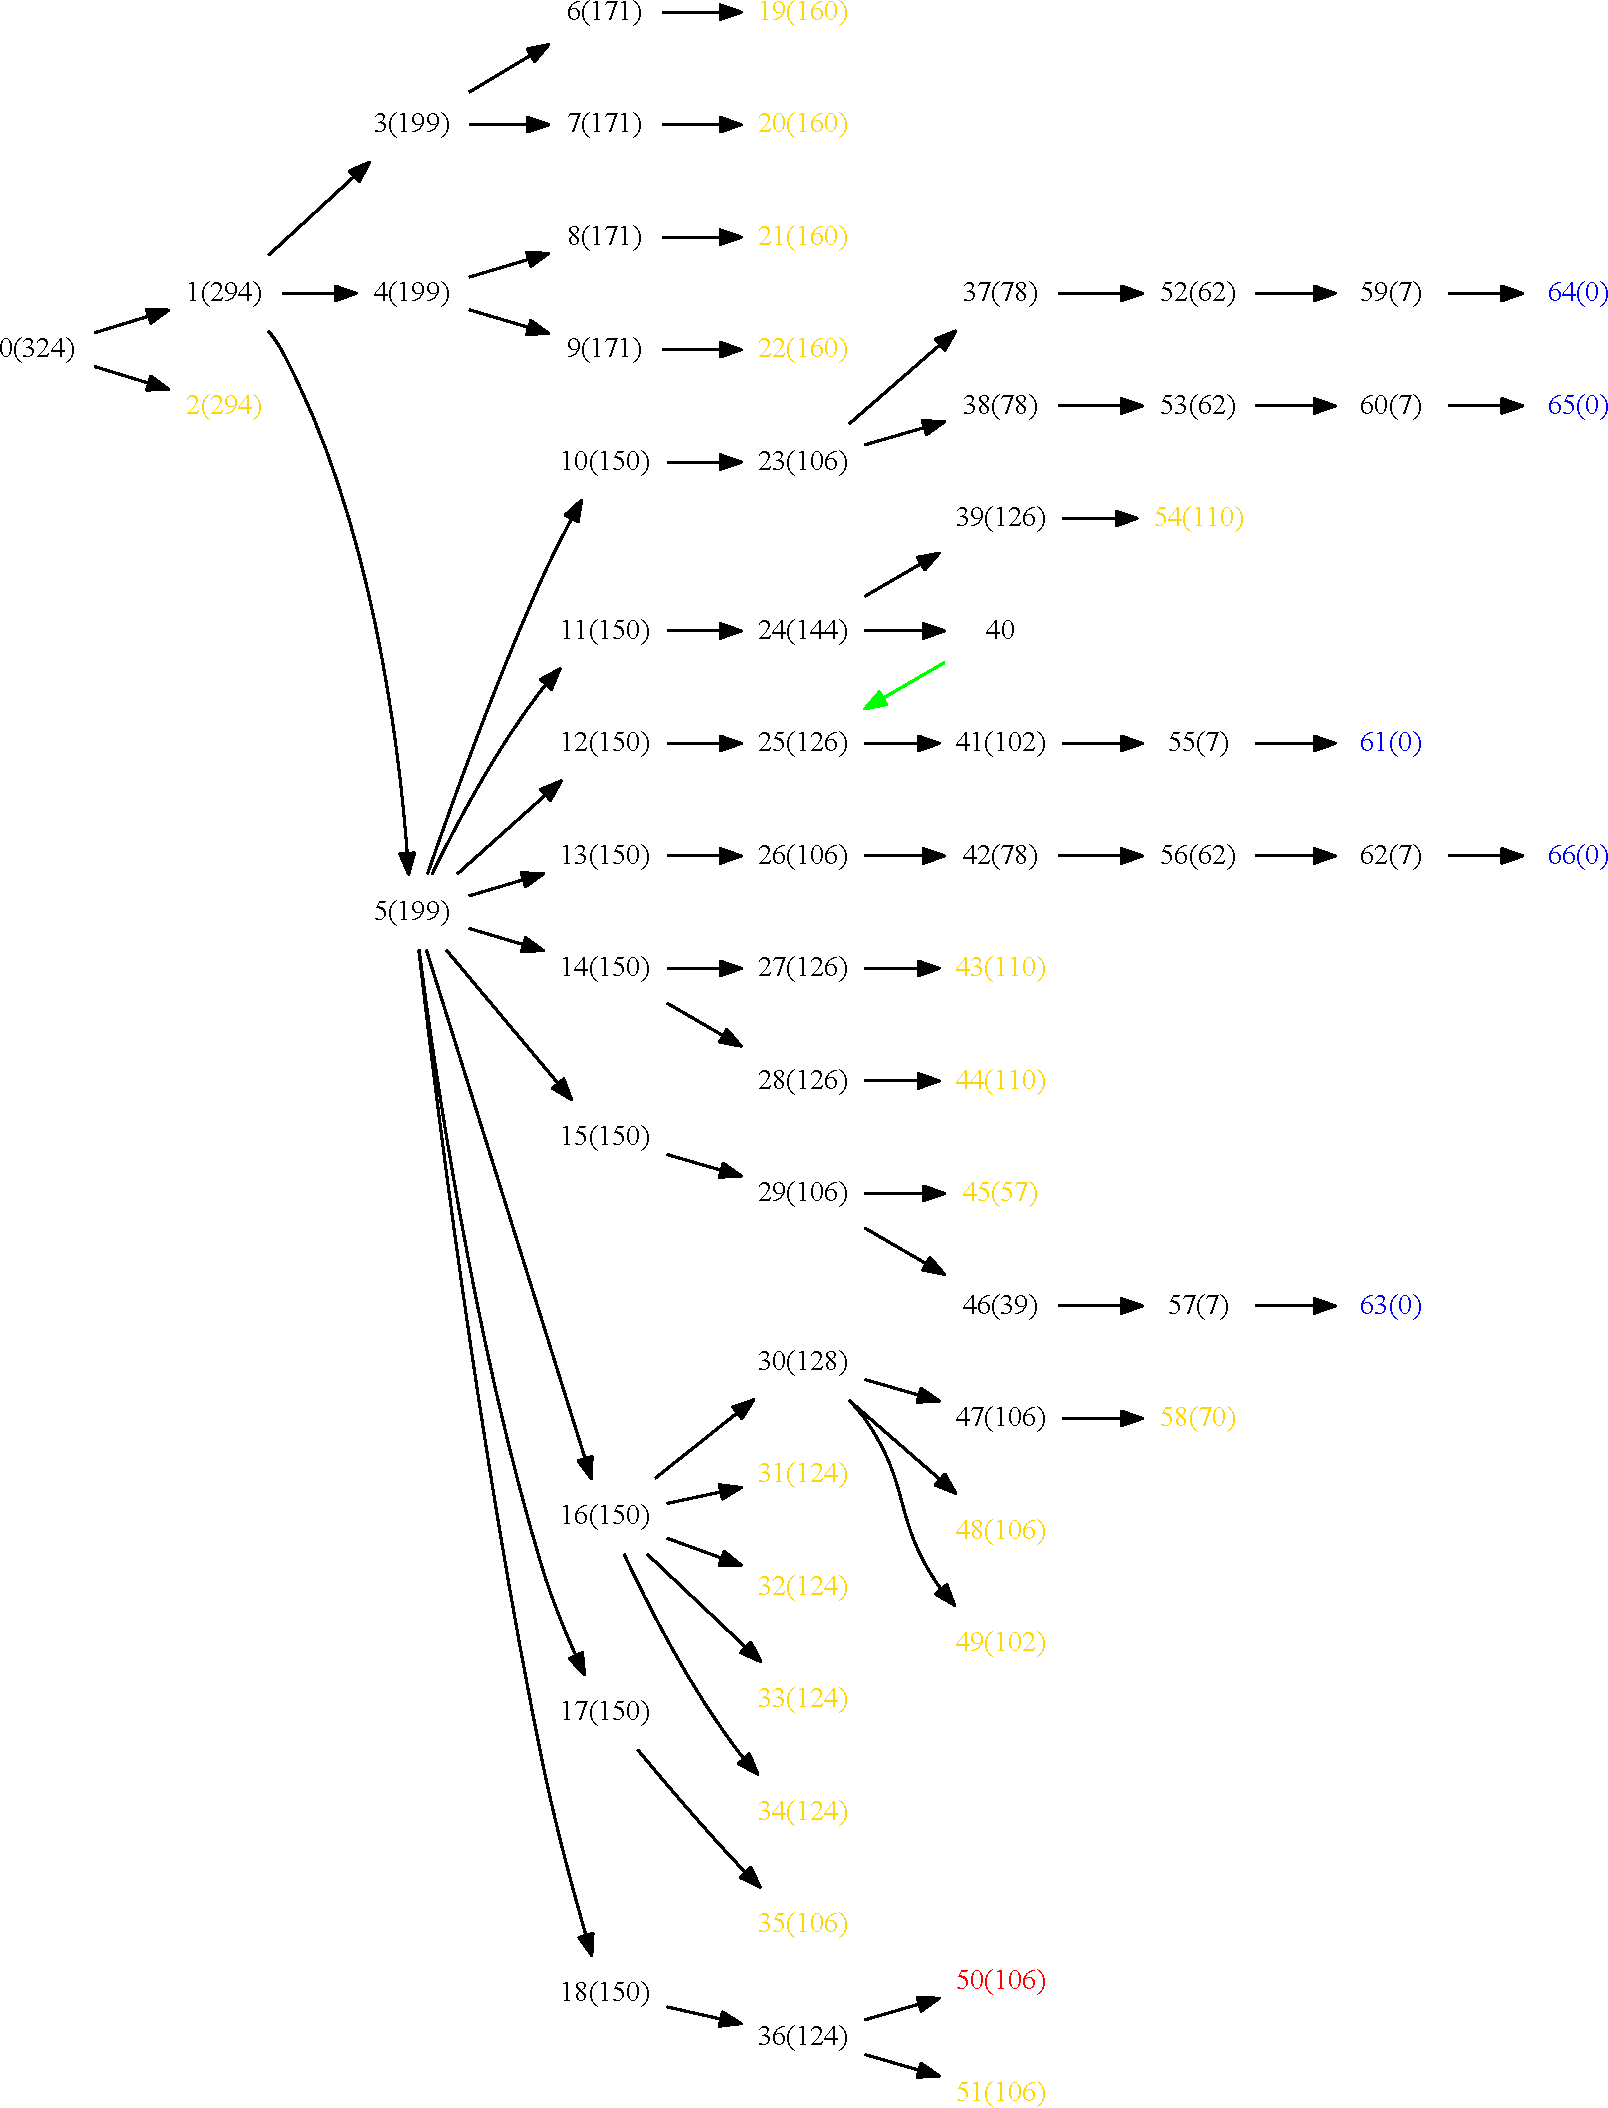
\includegraphics[width=\textwidth]{fig/2S1L-dir-number.pdf}
\caption{2S-1L 直接求解的分支图}\label{sb2-d}
\end{figure}

两种解法有两个共同的解
\begin{equation}
\renewcommand{\arraystretch}{1.2}
\left\{
\begin{array}{l}
{{p}_{11}}=0,
{{p}_{13}}=-{{p}_{14}},
{{p}_{22}}=\frac{{{p}_{12}}\,{{p}_{24}}}{{{p}_{14}}},
{{p}_{23}}=-{{p}_{24}},
{{p}_{31}}=0,\\
{{p}_{32}}=-\frac{\alpha\,{{{p}_{21}}}^{2}}{{{{p}_{14}}}^{2}\,{{p}_{12}}},
{{p}_{33}}=\frac{\alpha\,{{{p}_{21}}}^{2}}{{{{p}_{12}}}^{2}\,{{p}_{14}}},
{{p}_{34}}=-\frac{\alpha\,{{{p}_{21}}}^{2}}{{{{p}_{12}}}^{2}\,{{p}_{14}}},
{{p}_{41}}=\frac{3\,\alpha\,{{p}_{21}}\,{{p}_{24}}}{2\,{{p}_{14}}},\\ 
{{p}_{42}}=\frac{3\,\alpha\,\left( {{{p}_{12}}}^{2}\,{{{p}_{24}}}^{2}-{{{p}_{14}}}^{2}\,{{{p}_{21}}}^{2}\right) }{4\,{{{p}_{14}}}^{2}\,{{p}_{12}}},
{{p}_{43}}=-\frac{\left( 3\,{{{p}_{12}}}^{2}\,{{{p}_{24}}}^{2}-{{{p}_{14}}}^{2}\,{{{p}_{21}}}^{2}\right) \,\alpha}{4\,{{{p}_{12}}}^{2}\,{{p}_{14}}},\\
{{p}_{44}}=\frac{\left( 3\,{{{p}_{12}}}^{2}\,{{{p}_{24}}}^{2}-{{{p}_{14}}}^{2}\,{{{p}_{21}}}^{2}\right) \,\alpha}{4\,{{{p}_{12}}}^{2}\,{{p}_{14}}},
{{q}_{1}}=\frac{{{{p}_{12}}}^{2}}{{{{p}_{14}}}^{2}},
{{q}_{4}}=\frac{{{{p}_{14}}}^{2}\,{{q}_{2}}\,{{q}_{3}}}{{{{p}_{12}}}^{2}}
\end{array}
\right\}
\end{equation}
和
\begin{equation}
\renewcommand{\arraystretch}{1.2}
\left\{
\begin{array}{l}
{{p}_{12}}=0,
{{p}_{13}}=-\frac{{{p}_{11}}\,{{p}_{24}}}{{{p}_{21}}},
{{p}_{14}}=\frac{{{p}_{11}}\,{{p}_{24}}}{{{p}_{21}}},
{{p}_{23}}=-{{p}_{24}},
{{p}_{31}}=-\frac{\alpha\,{{{p}_{22}}}^{2}\,{{{p}_{21}}}^{2}}{{{{p}_{24}}}^{2}\,{{{p}_{11}}}^{3}},
{{p}_{32}}=0,\\ 
{{p}_{33}}=\frac{{{p}_{21}}\,\alpha\,{{{p}_{22}}}^{2}}{{{{p}_{11}}}^{3}\,{{p}_{24}}},
{{p}_{34}}=-\frac{{{p}_{21}}\,\alpha\,{{{p}_{22}}}^{2}}{{{{p}_{11}}}^{3}\,{{p}_{24}}},
{{p}_{41}}=\frac{3\,\alpha\,\left( {{{p}_{21}}}^{2}-{{{p}_{22}}}^{2}\right) }{4\,{{p}_{11}}},
{{p}_{42}}=\frac{3\,\alpha\,{{p}_{21}}\,{{p}_{22}}}{2\,{{p}_{11}}},\\ 
{{p}_{43}}=-\frac{{{p}_{24}}\,\left( 3\,{{{p}_{21}}}^{2}-{{{p}_{22}}}^{2}\right) \,\alpha}{4\,{{p}_{11}}\,{{p}_{21}}},
{{p}_{44}}=\frac{{{p}_{24}}\,\left( 3\,{{{p}_{21}}}^{2}-{{{p}_{22}}}^{2}\right) \,\alpha}{4\,{{p}_{11}}\,{{p}_{21}}},
{{q}_{1}}=\frac{{{{p}_{21}}}^{2}}{{{{p}_{24}}}^{2}},
{{q}_{4}}=\frac{{{{p}_{24}}}^{2}\,{{q}_{2}}\,{{q}_{3}}}{{{{p}_{21}}}^{2}}
\end{array}
\right\} . 
\end{equation}

直接求解特有的三个解为
\begin{equation}
\renewcommand{\arraystretch}{1.2}
\left\{
\begin{array}{l}
{{p}_{11}}=-\frac{3\,\alpha\,{{{p}_{22}}}^{2}\,{{p}_{41}}}{\left( 4\,{{{p}_{41}}}^{2}+4\,{{{p}_{42}}}^{2}\right) },
{{p}_{12}}=\frac{3\,\alpha\,{{{p}_{22}}}^{2}\,{{p}_{42}}}{\left( 4\,{{{p}_{41}}}^{2}+4\,{{{p}_{42}}}^{2}\right) },
{{p}_{13}}=-\frac{3\,\alpha\,{{p}_{22}}\,{{p}_{24}}}{4\,{{p}_{42}}},
{{p}_{14}}=\frac{3\,\alpha\,{{p}_{22}}\,{{p}_{24}}}{4\,{{p}_{42}}},\\ 
{{p}_{23}}=-{{p}_{24}},
{{p}_{31}}=\frac{64\,{{{p}_{41}}}^{3}\,{{{p}_{42}}}^{2}}{27\,{\alpha}^{2}\,{{{p}_{22}}}^{2}\,{{{p}_{24}}}^{2}\,\left( {{{p}_{41}}}^{2}+{{{p}_{42}}}^{2}\right) },
{{p}_{32}}=-\frac{64\,{{{p}_{41}}}^{2}\,{{{p}_{42}}}^{3}}{27\,{\alpha}^{2}\,{{{p}_{22}}}^{2}\,{{{p}_{24}}}^{2}\,\left( {{{p}_{41}}}^{2}+{{{p}_{42}}}^{2}\right) },\\ 
{{p}_{21}}=0,
{{p}_{33}}=\frac{64\,{{{p}_{41}}}^{2}\,{{p}_{42}}}{27\,{\alpha}^{2}\,{{p}_{24}}\,{{{p}_{22}}}^{3}},
{{p}_{34}}=-\frac{64\,{{{p}_{41}}}^{2}\,{{p}_{42}}}{27\,{\alpha}^{2}\,{{p}_{24}}\,{{{p}_{22}}}^{3}},
{{p}_{43}}=\frac{{{p}_{24}}\,\left( {{{p}_{41}}}^{2}-3\,{{{p}_{42}}}^{2}\right) }{3\,{{p}_{42}}\,{{p}_{22}}},\\ 
{{p}_{44}}=-\frac{{{p}_{24}}\,\left( {{{p}_{41}}}^{2}-3\,{{{p}_{42}}}^{2}\right) }{3\,{{p}_{42}}\,{{p}_{22}}},
{{q}_{1}}=\frac{{{{p}_{22}}}^{2}\,{{{p}_{42}}}^{2}}{{{{p}_{24}}}^{2}\,\left( {{{p}_{41}}}^{2}+{{{p}_{42}}}^{2}\right) },
{{q}_{4}}=\frac{{{q}_{2}}\,{{q}_{3}}\,{{{p}_{24}}}^{2}\,\left( {{{p}_{41}}}^{2}+{{{p}_{42}}}^{2}\right) }{{{{p}_{22}}}^{2}\,{{{p}_{42}}}^{2}}
\end{array}
\right\} ,
\end{equation}
\begin{equation}
\renewcommand{\arraystretch}{1.2}
\left\{
\begin{array}{l}
{{p}_{11}}=\frac{{{p}_{14}}\,{{p}_{21}}}{{{p}_{24}}},
% {{p}_{12}}=0,
% {{p}_{52}}=0,
% {{p}_{32}}=0,
p_{12}=p_{32}=p_{52}=0,
{{p}_{13}}=-{{p}_{14}},
{{p}_{23}}=-{{p}_{24}},
{{p}_{31}}=-\frac{{{{p}_{22}}}^{2}\,{{p}_{24}}\,\alpha}{{{{p}_{14}}}^{3}\,{{p}_{21}}},\\ 
{{p}_{33}}=\frac{{{{p}_{22}}}^{2}\,{{{p}_{24}}}^{2}\,\alpha}{{{{p}_{21}}}^{2}\,{{{p}_{14}}}^{3}},
{{p}_{34}}=-\frac{{{{p}_{22}}}^{2}\,{{{p}_{24}}}^{2}\,\alpha}{{{{p}_{21}}}^{2}\,{{{p}_{14}}}^{3}},
{{p}_{41}}=\frac{3\,{{p}_{24}}\,\alpha\,\left( {{{p}_{21}}}^{2}-{{{p}_{22}}}^{2}\right) }{4\,{{p}_{14}}\,{{p}_{21}}},
{{p}_{42}}=\frac{3\,\alpha\,{{p}_{22}}\,{{p}_{24}}}{2\,{{p}_{14}}},\\ 
{{p}_{43}}=-\frac{{{{p}_{24}}}^{2}\,\left( 3\,{{{p}_{21}}}^{2}-{{{p}_{22}}}^{2}\right) \,\alpha}{4\,{{{p}_{21}}}^{2}\,{{p}_{14}}},
{{p}_{44}}=\frac{{{{p}_{24}}}^{2}\,\left( 3\,{{{p}_{21}}}^{2}-{{{p}_{22}}}^{2}\right) \,\alpha}{4\,{{{p}_{21}}}^{2}\,{{p}_{14}}},
{{q}_{1}}=\frac{{{{p}_{21}}}^{2}}{{{{p}_{24}}}^{2}},
{{q}_{4}}=\frac{{{{p}_{24}}}^{2}\,{{q}_{2}}\,{{q}_{3}}}{{{{p}_{21}}}^{2}},
\end{array}
\right\}
\end{equation}
和
\begin{equation}
\renewcommand{\arraystretch}{1.2}
\left\{
\begin{array}{l}
{{p}_{11}}=\frac{3\,{{p}_{14}}\,\left( 3\,\alpha\,{{{p}_{21}}}^{2}\,{{p}_{24}}-3\,\alpha\,{{{p}_{22}}}^{2}\,{{p}_{24}}+4\,{{p}_{14}}\,{{p}_{22}}\,{{p}_{42}}\right) \,{{p}_{21}}\,\alpha}{\left( 9\,{\alpha}^{2}\,{{{p}_{21}}}^{2}\,{{{p}_{24}}}^{2}+9\,{\alpha}^{2}\,{{{p}_{22}}}^{2}\,{{{p}_{24}}}^{2}-24\,\alpha\,{{p}_{14}}\,{{p}_{22}}\,{{p}_{24}}\,{{p}_{42}}+16\,{{{p}_{14}}}^{2}\,{{{p}_{42}}}^{2}\right) },\\ 
{{p}_{12}}=\frac{6\,{{p}_{14}}\,\left( 3\,\alpha\,{{p}_{22}}\,{{p}_{24}}-2\,{{p}_{14}}\,{{p}_{42}}\right) \,{{{p}_{21}}}^{2}\,\alpha}{\left( 9\,{\alpha}^{2}\,{{{p}_{21}}}^{2}\,{{{p}_{24}}}^{2}+9\,{\alpha}^{2}\,{{{p}_{22}}}^{2}\,{{{p}_{24}}}^{2}-24\,\alpha\,{{p}_{14}}\,{{p}_{22}}\,{{p}_{24}}\,{{p}_{42}}+16\,{{{p}_{14}}}^{2}\,{{{p}_{42}}}^{2}\right) },\\
{{p}_{31}}=-\frac{\left( 3\,\alpha\,{{p}_{22}}\,{{p}_{24}}-4\,{{p}_{14}}\,{{p}_{42}}\right) ^{2}\,\left( 3\,\alpha\,{{{p}_{21}}}^{2}\,{{p}_{24}}-3\,\alpha\,{{{p}_{22}}}^{2}\,{{p}_{24}}+4\,{{p}_{14}}\,{{p}_{22}}\,{{p}_{42}}\right) }{3\,{{{p}_{14}}}^{3}\,\left( 9\,{\alpha}^{2}\,{{{p}_{21}}}^{2}\,{{{p}_{24}}}^{2}+9\,{\alpha}^{2}\,{{{p}_{22}}}^{2}\,{{{p}_{24}}}^{2}-24\,\alpha\,{{p}_{14}}\,{{p}_{22}}\,{{p}_{24}}\,{{p}_{42}}+16\,{{{p}_{14}}}^{2}\,{{{p}_{42}}}^{2}\right) \,{{p}_{21}}},\\
{{p}_{32}}=-\frac{2\,\left( 3\,\alpha\,{{p}_{22}}\,{{p}_{24}}-2\,{{p}_{14}}\,{{p}_{42}}\right) \,\left( 3\,\alpha\,{{p}_{22}}\,{{p}_{24}}-4\,{{p}_{14}}\,{{p}_{42}}\right) ^{2}}{3\,{{{p}_{14}}}^{3}\,\left( 9\,{\alpha}^{2}\,{{{p}_{21}}}^{2}\,{{{p}_{24}}}^{2}+9\,{\alpha}^{2}\,{{{p}_{22}}}^{2}\,{{{p}_{24}}}^{2}-24\,\alpha\,{{p}_{14}}\,{{p}_{22}}\,{{p}_{24}}\,{{p}_{42}}+16\,{{{p}_{14}}}^{2}\,{{{p}_{42}}}^{2}\right) },\\ 
{{p}_{33}}=\frac{\left( 3\,\alpha\,{{p}_{22}}\,{{p}_{24}}-4\,{{p}_{14}}\,{{p}_{42}}\right) ^{2}}{9\,{{{p}_{21}}}^{2}\,\alpha\,{{{p}_{14}}}^{3}},
{{p}_{34}}=-\frac{\left( 3\,\alpha\,{{p}_{22}}\,{{p}_{24}}-4\,{{p}_{14}}\,{{p}_{42}}\right) ^{2}}{9\,{{{p}_{21}}}^{2}\,\alpha\,{{{p}_{14}}}^{3}},\\ 
{{p}_{41}}=\frac{\left( 3\,\alpha\,{{{p}_{21}}}^{2}\,{{p}_{24}}+3\,\alpha\,{{{p}_{22}}}^{2}\,{{p}_{24}}-4\,{{p}_{14}}\,{{p}_{22}}\,{{p}_{42}}\right) }{4\,{{p}_{14}}\,{{p}_{21}}},
{{p}_{13}}=-{{p}_{14}},
{{p}_{23}}=-{{p}_{24}},\\ 
{{p}_{43}}=\frac{\left( -27\,{\alpha}^{2}\,{{{p}_{21}}}^{2}\,{{{p}_{24}}}^{2}+9\,{\alpha}^{2}\,{{{p}_{22}}}^{2}\,{{{p}_{24}}}^{2}-24\,\alpha\,{{p}_{14}}\,{{p}_{22}}\,{{p}_{24}}\,{{p}_{42}}+16\,{{{p}_{14}}}^{2}\,{{{p}_{42}}}^{2}\right) }{36\,{{{p}_{21}}}^{2}\,\alpha\,{{p}_{14}}},\\ 
{{p}_{44}}=\frac{\left( 27\,{\alpha}^{2}\,{{{p}_{21}}}^{2}\,{{{p}_{24}}}^{2}-9\,{\alpha}^{2}\,{{{p}_{22}}}^{2}\,{{{p}_{24}}}^{2}+24\,\alpha\,{{p}_{14}}\,{{p}_{22}}\,{{p}_{24}}\,{{p}_{42}}-16\,{{{p}_{14}}}^{2}\,{{{p}_{42}}}^{2}\right) }{36\,{{{p}_{21}}}^{2}\,\alpha\,{{p}_{14}}},\\ 
{{q}_{1}}=\frac{9\,{\alpha}^{2}\,{{{p}_{21}}}^{2}\,\left( {{{p}_{21}}}^{2}+{{{p}_{22}}}^{2}\right) }{\left( 9\,{\alpha}^{2}\,{{{p}_{21}}}^{2}\,{{{p}_{24}}}^{2}+9\,{\alpha}^{2}\,{{{p}_{22}}}^{2}\,{{{p}_{24}}}^{2}-24\,\alpha\,{{p}_{14}}\,{{p}_{22}}\,{{p}_{24}}\,{{p}_{42}}+16\,{{{p}_{14}}}^{2}\,{{{p}_{42}}}^{2}\right) },\\ 
{{q}_{4}}=\frac{{{q}_{2}}\,{{q}_{3}}\,\left( 9\,{\alpha}^{2}\,{{{p}_{21}}}^{2}\,{{{p}_{24}}}^{2}+9\,{\alpha}^{2}\,{{{p}_{22}}}^{2}\,{{{p}_{24}}}^{2}-24\,\alpha\,{{p}_{14}}\,{{p}_{22}}\,{{p}_{24}}\,{{p}_{42}}+16\,{{{p}_{14}}}^{2}\,{{{p}_{42}}}^{2}\right) }{9\,{\alpha}^{2}\,{{{p}_{21}}}^{2}\,\left( {{{p}_{21}}}^{2}+{{{p}_{22}}}^{2}\right) }
\end{array}
\right\} . \label{2S1L-eq}
\end{equation} 

继承求解特有的解为 
\begin{equation}
\renewcommand{\arraystretch}{1.2}
\left\{
\begin{array}{l}
{{p}_{13}}=-{{p}_{14}},
{{p}_{21}}=\frac{\left( {{{p}_{11}}}^{2}\,{{p}_{24}}+{{{p}_{12}}}^{2}\,{{p}_{24}}-{{p}_{12}}\,{{p}_{14}}\,{{p}_{22}}\right) }{{{p}_{11}}\,{{p}_{14}}},
{{p}_{23}}=-{{p}_{24}},\\
{{p}_{32}}=-\frac{{{p}_{12}}\,\alpha\,\left( {{p}_{12}}\,{{p}_{24}}-{{p}_{14}}\,{{p}_{22}}\right) ^{2}}{{{{p}_{11}}}^{2}\,{{{p}_{14}}}^{4}},
{{p}_{33}}=\frac{\alpha\,\left( {{p}_{12}}\,{{p}_{24}}-{{p}_{14}}\,{{p}_{22}}\right) ^{2}}{{{{p}_{11}}}^{2}\,{{{p}_{14}}}^{3}},
{{p}_{34}}=-\frac{\alpha\,\left( {{p}_{12}}\,{{p}_{24}}-{{p}_{14}}\,{{p}_{22}}\right) ^{2}}{{{{p}_{11}}}^{2}\,{{{p}_{14}}}^{3}},\\
{{p}_{41}}=\frac{3\,\alpha\,\left( {{{p}_{11}}}^{2}\,{{{p}_{24}}}^{2}+{{{p}_{12}}}^{2}\,{{{p}_{24}}}^{2}-{{{p}_{14}}}^{2}\,{{{p}_{22}}}^{2}\right) }{4\,{{p}_{11}}\,{{{p}_{14}}}^{2}},
{{p}_{31}}=-\frac{\alpha\,\left( {{p}_{12}}\,{{p}_{24}}-{{p}_{14}}\,{{p}_{22}}\right) ^{2}}{{{p}_{11}}\,{{{p}_{14}}}^{4}},\\
{{p}_{42}}=-\frac{3\,\alpha\,\left( {{{p}_{11}}}^{2}\,{{p}_{12}}\,{{{p}_{24}}}^{2}-2\,{{{p}_{11}}}^{2}\,{{p}_{14}}\,{{p}_{22}}\,{{p}_{24}}+{{{p}_{12}}}^{3}\,{{{p}_{24}}}^{2}-2\,{{{p}_{12}}}^{2}\,{{p}_{14}}\,{{p}_{22}}\,{{p}_{24}}+{{p}_{12}}\,{{{p}_{14}}}^{2}\,{{{p}_{22}}}^{2}\right) }{4\,{{{p}_{11}}}^{2}\,{{{p}_{14}}}^{2}},\\ 
{{p}_{43}}=-\frac{\alpha\,\left( 3\,{{{p}_{11}}}^{2}\,{{{p}_{24}}}^{2}-{{{p}_{12}}}^{2}\,{{{p}_{24}}}^{2}+2\,{{p}_{12}}\,{{p}_{14}}\,{{p}_{22}}\,{{p}_{24}}-{{{p}_{14}}}^{2}\,{{{p}_{22}}}^{2}\right) }{4\,{{{p}_{11}}}^{2}\,{{p}_{14}}},
{{q}_{1}}=\frac{\left( {{{p}_{11}}}^{2}+{{{p}_{12}}}^{2}\right) }{{{{p}_{14}}}^{2}},\\ 
{{p}_{44}}=\frac{\alpha\,\left( 3\,{{{p}_{11}}}^{2}\,{{{p}_{24}}}^{2}-{{{p}_{12}}}^{2}\,{{{p}_{24}}}^{2}+2\,{{p}_{12}}\,{{p}_{14}}\,{{p}_{22}}\,{{p}_{24}}-{{{p}_{14}}}^{2}\,{{{p}_{22}}}^{2}\right) }{4\,{{{p}_{11}}}^{2}\,{{p}_{14}}},
{{q}_{2}}=\frac{{{q}_{4}}\,\left( {{{p}_{11}}}^{2}+{{{p}_{12}}}^{2}\right) }{{{{p}_{14}}}^{2}\,{{q}_{3}}}
\end{array}
\right\}. \label{2S1L-plot}
\end{equation}

经验证, 我们发现\refeqn{2S1L-eq}和\refeqn{2S1L-plot}是等价的. 所以, 直接求解比继承求解多解得两个解, 且直接求解的结果形式更复杂\D 用时更长. 所以, 在对解的完整性要求不严格时, 继承求解是更优的选择.

对于\refeqn{2S1L-plot} 我们取 $t=0,z=0,p_{12}=-1,p_{14}=1/2,p_{22}=-2,p_{24}=1/10,q_4=1/100,\alpha=p_{11}=p_{51}=p_{52}=q_3=1$进行绘图, 结果如\reffig{fig-2S1L}所示. 可以看出这是两个扭状孤子和一个 lump 的相互作用解.

\begin{figure}[H]
\centering
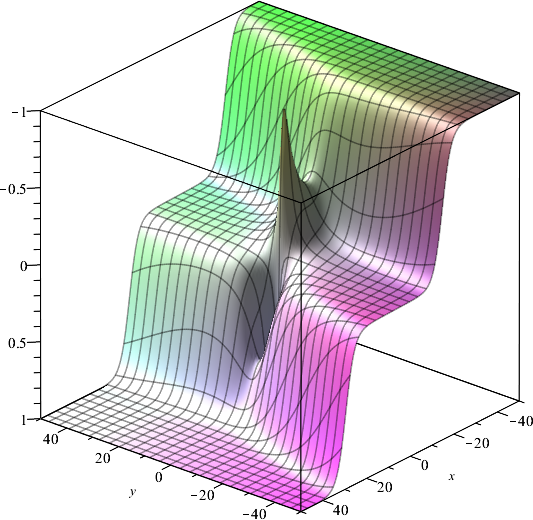
\includegraphics[width=.6\textwidth]{fig/2S1L.png}
\caption{(3+1)JM 方程的 2S-1L 解} \label{fig-2S1L}
\end{figure}

\subsection{求解效率对比}

现在, 本文将对比 PGSolve 和 Maple 内置求解函数的效率. 一般而言, 我们会利用 Maple 的\cd{solve}函数进行方程组的求解. 但是, 对于 NS1L 所产生的问题, 即使只有 20 个方程, \cd{solve}也不能完成求解. 对于 (2+1)SK 方程的 0S-1L 解产生的 20 个方程, 本文作者在实验中等待了超过 72 小时仍未得到该方程组的解. 但是, Maple 内置的 \cd{PDEtools[Solve]} 函数却能在几秒内完成求解. 这显然是\cd{solve}函数的一个 BUG.因此, 本文将对比 PGSolve 和 \cd{PDEtools[Solve]} 的求解效率, 实验结果如\reftab{NS1L-cmp}所示. 

\begin{table}[htbp]
\centering
\caption{PGSolve 和 PDEtools[Solve] 的运行时间对比表} \label{NS1L-cmp}
\begin{tabular}{cccccc}
\hline
来源方程 & 阶数 & 方程数 & 变量数 & PGSolve用时 & Solve用时 \\
\hline
(2+1)SK & 0 & 20 & 9 & 0.724 & 3.483 \\
(2+1)BKP-T & 0 & 20 & 9 & 0.571 & 3.486 \\
(2+1)KP & 0 & 35 & 9 & 1.759 & 29.643 \\
(3+1)YTSF & 0 & 35 & 11 & 1.229 & 8.839 \\
(3+1)JM & 0 & 35 & 11 & 0.845 & >1800 \\
(2+1)SK & 1 & 65 & 13 & 10.241 & >1800 \\
(3+1)YTSF & 1 & 120 & 16 & 12.228 & 1696.852 \\
\hline
\end{tabular}
\end{table}

在\reftab{NS1L-cmp}中, 我们选择了几个不同规模的问题进行测试. 可以看出, 对于只有20个方程的方程组, PGSolve 的求解时间在 1 秒以内, 而 \cd{PDEtools[Solve]} 的用时则在 3 秒左右, PGSolve 的优势不是很大. 但当方程数量增加到 35 个时, \cd{PDEtools[Solve]} 的求解时间则大幅增加, 其中一个例子用时约 10 秒, 另一个例子用时 30 秒, 甚至有一个例子在 1800 内无法完成求解. 但是, 对于 35 个方程的例子, PGSolve 的求解时间仍在 1 秒左右. 对于 65 个方程的例子, PGSolve 的求解时间约为 10 秒, 而\cd{PDEtools[Solve]}则不能在1800内完成求解. 表中规模最大的例子有120个方程, PGSolve 在 10 秒左右完成了求解, \cd{PDEtools[Solve]}则用时约 1700 秒. 所以, 对于规模在 100 以上的方程组, PGSolve 的求解效率比 \cd{PDEtools[Solve]} 高 100 倍以上.

因为\reftab{NS1L-cmp}中的例子仍没有触及到 PGSolve 的性能边界, 所以我们在\reftab{NS1L-tb}中选择了一些方程对 PGSolve 进行进一步的测试. 在\reftab{NS1L-cmp}中, 为了公平地进行对比, PGSolve 采用的是直接求解的方式, 而\reftab{NS1L-tb}中所有的高阶解都是通过继承求解得到的. \reftab{NS1L-tb}中统计的运行时间包含了生成方程组\D 求解方程组和过滤等价解这三个步骤, 所以这里(3+1)YTSF方程的相关运行时间略长与上文描述的运行时间. 此外, (2+1)SK方程和(2+1)BKP-T方程在求 1S-1L 解时分组大小是3, 这是因为分组大小为5时会无解. 关于这两个方程还有一个有趣的结论: 这两个方程的 TPE 都有两组解, 取第一个 TPE 时 lump 对应的方程有20个且有解, 取第二个 TPE 时 lump 解对应的方程有 120 个且无解. 这和 TwSolver 求解的结果是一致的. 

\begin{table}[htbp]
\centering
\caption{NS1L运行结果汇总} \label{NS1L-tb}
\begin{tabular}{cccccc}
\hline
方程名称    & 解的阶数 & 方程数量 & 分组大小 & 解的个数 & 运行时间(s) \\ 
\hline 
(2+1)SK & 0 & 20 & 5 & 1 & 1.875 \\
(2+1)SK & 1 & 65 & 3 & 1 & 3.154 \\
(2+1)SK & 2 & 179 & 5 & 2 & 12.926 \\
(2+1)BKP-T & 0 & 20 & 5 & 1 & 1.036 \\
(2+1)BKP-T & 1 & 65 & 3 & 1 & 3.181 \\
(2+1)BKP-T & 2 & 179 & 5 & 2 & 12.749 \\
(3+1)YTSF & 0 & 35 & 5 & 3 & 2.891 \\
(3+1)YTSF & 1 & 120 & 5 & 3 & 8.713 \\
(3+1)YTSF & 2 & 324 & 5 & 3 & 38.527 \\
(3+1)JM & 0 & 35 & 5 & 4 & 3.120 \\
(3+1)JM & 1 & 120 & 5 & 6 & 14.910 \\
(3+1)JM & 2 & 324 & 5 & 5 & 81.711 \\
\hline 
\end{tabular}
\end{table}

从\reftab{NS1L-tb}中可以看出, 采用继承求解的方式, 对于30个左右的方程, PGSolve 能在几秒内完成求解; 对于 100 个左右的方程, PGSolve 能在十几秒内完成求解; 对于 300 个左右的方程, PGSolve 能够在几十秒内完成求解. 
 

\section{小结}
在本章中, 我们提出了一个分组并行的算法来求解大规模代数方程组, 并将其实现为 PGSolve 软件包. 作为 PGSolve 的应用实例, 我们编写了用直接代数方法求$n$孤子-1 lump相互作用解的软件包 NS1L. 除了直接对输入方程进行求解之外, PGSolve 还支持自行设定初始解进行求解, 这种方法被称为是继承求解. 在 NS1L 中, 将低阶解作为高阶解的初始解进行求解, 能够极大的提升求解的效率. 基于继承求解, 我们能够在几十秒内求解含300个左右方程的方程组, 其效率在普通求解函数的 100 以上. 

此外, 关于 PGSolve 的使用, 本文总结了以下几点建议:
\begin{compactenum}[(1)]
\item PGSolve 不能保证获得所有满足要求的解, 它是通过牺牲解的完整性来提升求解效率的.
\item 继承求解能够极大地提升求解效率. 对于一些有包含关系的方程组, 可以先求解小规模的方程组, 再将小规模方程的解作为大规模方程组的初始解进行求解. 
\item 在继承求解时, 不一定要将所有的解都作为初始解, 也可以选择一部分形式较为简单的解作为初始解.
\item 调整分组大小将会影响求解的效率和结果. 当单步求解的时间过长时, 应该减小分组大小; 当求解的分支过多时, 应该增加分组大小. 当无解时, 也可以尝试改变分组大小重新求解. 
\end{compactenum}
 
本章的研究成果是本文新增的工作, 暂未向期刊投稿. 
